\documentclass[a4paper,12pt]{article}

\usepackage[utf8]{inputenc}
\usepackage{graphicx}
\usepackage{xcolor} 
\usepackage[cm]{fullpage}
\usepackage{bold-extra} % to get rid of some warnings
\usepackage{bm}
\usepackage{amssymb}
\usepackage{upgreek}
\usepackage{amsmath}
\usepackage{listings}

\usepackage{hyperref}
\hypersetup{
colorlinks,
citecolor=black,
filecolor=black,
linkcolor=violet,
urlcolor=black}

\usepackage[colorinlistoftodos,prependcaption,textsize=tiny]{todonotes}


\lstset{ 
  language=Python,
  backgroundcolor=\color{white},   % choose the background color; you must add \usepackage{xcolor}; should come as last argument
  basicstyle=\footnotesize,        % the size of the fonts that are used for the code
  breakatwhitespace=false,         % sets if automatic breaks should only happen at whitespace
  breaklines=true,                 % sets automatic line breaking
  captionpos=b,                    % sets the caption-position to bottom
  frame=single,                    % adds a frame around the code
  keepspaces=true,                 % keeps spaces in text, useful for keeping indentation of code 
  keywordstyle=\color{blue},       % keyword style
}

\newcommand{\aspect}{{\textsc{Aspect~}{}}}
\newcommand{\elefant}{{\textsc{Elefant~}{}}}
\newcommand{\citcoms}{{\textsc{CitcomS~}{}}}
\newcommand{\citcomsve}{{\textsc{CitcomSVE~}{}}}
\newcommand{\fantom}{{\textsc{Fantom~}{}}}
\newcommand{\sulec}{{\textsc{Sulec~}{}}}
\newcommand{\sopale}{{\textsc{Sopale~}{}}}
\newcommand{\douar}{{\textsc{Douar~}{}}}
\newcommand{\ghost}{{\textsc{Ghost~}{}}}
\newcommand{\fluidity}{{\textsc{Fluidity~}{}}}
\newcommand{\sepran}{{\textsc{Sepran~}{}}}
\newcommand{\stone}{{\color{teal} {\textsc{stone~}}}}
\newcommand{\etal}{{\it et al.~}}
\newcommand{\nn}{\nonumber}
\newcommand{\A}{{\mathbb{A}}}
\newcommand{\K}{{\mathbb{K}}}
\newcommand{\J}{{\mathbb{J}}}
\newcommand{\G}{{\mathbb{G}}}
\newcommand{\Z}{{\mathbb{Z}}}
\newcommand{\C}{{\mathbb{C}}}
\newcommand{\W}{{\mathbb{W}}}
\newcommand{\R}{{\mathbb{R}}}
\newcommand{\M}{{\mathbb{M}}}
\newcommand{\N}{{\mathbb{N}}}
\newcommand{\LLL}{{\mathbb{L}}}
\newcommand{\SSS}{{\mathbb{S}}}
\newcommand{\HH}{{\mathbb{H}}}
\newcommand{\Literature}{\includegraphics[height=4mm]{images/lit} {\sffamily Relevant Literature}}
\newcommand{\bscthesis}{{(\bf BSc Thesis)}}
\newcommand{\mscthesis}{{(\bf MSc Thesis)}}
\newcommand{\captionfont}{\tiny}
\newcommand{\pythonfile}{\color{blue} \sffamily }
\newcommand{\shellscriptfile}{\color{purple} \sffamily }
\newcommand{\asciifile}{\color{olive} \sffamily }
\newcommand{\OK}{{\bf OK}}
\newcommand{\filenamefont }{\sl }
\newcommand{\foldernamefont }{\it }
\newcommand{\codefont}{\bfseries\ttfamily}
\newcommand{\Ranb}{{\mathsf{Ra}}}
\newcommand{\Nunb}{{\mathsf{Nu}}}
\newcommand{\Prnb}{{\mathsf{Pr}}}
\newcommand{\Penb}{{\mathsf{Pe}}}
\newcommand{\Dinb}{{\mathsf{Di}}}
\newcommand{\python}{\color{darkgray} \sffamily }
\newcommand{\bN}{{\mathcal{N}}}
\newcommand{\qx}{\underset{\tiny x}{q}}
\newcommand{\qy}{\underset{\tiny y}{q}}
\newcommand{\nx}{\underset{\tiny x}{n}}
\newcommand{\ny}{\underset{\tiny y}{n}}
\newcommand{\qhx}{\underset{\tiny x}{q_h}}
\newcommand{\qhy}{\underset{\tiny y}{q_h}}
\newcommand{\qix}{\underset{\tiny x}{q_i}}
\newcommand{\qiy}{\underset{\tiny y}{q_i}}
\newcommand{\Tx}{\underset{\tiny x}{T}}
\newcommand{\Ty}{\underset{\tiny y}{T}}
\newcommand{\blueqx}{  {\color{blue} \underset{\tiny x}{q}  }  }
\newcommand{\blueqy}{  {\color{blue} \underset{\tiny y}{q}  }  }
\newcommand{\blueT}{  {\color{blue} T}  }
\newcommand{\brownT}{  {\color{brown} T}  }
\newcommand{\brownqx}{  {\color{brown} \underset{\tiny x}{q}  }  }
\newcommand{\brownqy}{  {\color{brown} \underset{\tiny y}{q}  }  }
\newcommand\norm[1]{\left\lVert#1\right\rVert}


\usepackage{amsthm}
\newtheorem*{remark}{Remark}

%Bibliography stuff
\usepackage[maxnames=6]{biblatex}
\addbibresource{biblio_geosciences.bib}

\title{ELEFANT 2.0}
\author{C. Thieulot}

%%%%%%%%%%%%%%%%%%%%%%%%%%%%%%%%%%%%%%%%%%%%%%%%%%%%%%%%%%%
\begin{document}

\thispagestyle{empty}

\begin{center}
\includegraphics[width=0.96\linewidth]{images/elefant/logo_elefant_draft2}\\
{\large ELEFANT 2.0}
\end{center}

\newpage

%\maketitle
\tableofcontents

\newpage

This version on \elefant is different than the one I built from 2012 until 2018.
It incorporates many features and contains many identical algorithms with the original 
one but in a more streamlined version. Also the number of (outer) solver types, marker projections, 
element types, geometries, etc ... has been greatly reduced. 

\begin{center}
\includegraphics[width=7cm]{images/elefant/logo_elefant_small}
\end{center}

This code is in Fortran because a) this is the language I know best; b) it is (really) fast;
c) the interface with MUMPS is seamless.  




%%%%%%%%%%%%%%%%%%%%%%%%%%%%%%%%%%
\section{Philosophy}
\begin{itemize}
\item readability
\item not memory efficient/optimised
\item object oriented fortran
\item using modules which contain 99\% of the arrays
\item export to vtu 
\item testing
\item similar notations to python codes of fieldstone
\end{itemize}

%%%%%%%%%%%%%%%%%%%%%%%%%%%%%%%%%%
\section{Principal features}

\begin{itemize}
\item physics:
\begin{itemize}
\item compressible and incompressible flow
\item visco-plastic rheology
\end{itemize}
\item 5 geometries:
\begin{itemize}
\item Cartesian box 2D
\item Cartesian box 3D
\item Annulus
\item Hollow Sphere
\item V. John 2D simplices
\end{itemize}
\item many FE element pairs:
\begin{itemize}
\item $Q_1\times P_0$
\item $Q_1^+\times Q_1$ (2D) and $Q_1^{++}\times Q_1$ (3D)
\item $Q_1^F \times P_0$ 
\item $Q_2\times Q_1$
\item $P_2 \times P_1$
\end{itemize}
\item Particle-in-Cell
\begin{itemize}
\item random or regular distribution of markers
\item paint  
\item elemental least square projection
\end{itemize}
\item penalty approach if $Q_1\times P_0$ used
\item Outer solver: Preconditioned Conjugate Gradients applied to Schur complement equation.
\item Inner solver: y12m, MUMPS or Preconditioned Conjugate Gradients.
\item free surface
\item open boundary conditions
\item Nonlinear rheologies (viscous-viscoplastic)
\item Newton solver (?)
\item implementation allows for nodes with only a component of velocity
\end{itemize}


\begin{center}
\begin{tabular}{|l|ccccc|}
\hline
       & cart 2D & cart 3D & annulus & shell & John\\
\hline
spaceV   & &&&& \\ 
$Q_1$    & \checkmark & \checkmark &\checkmark && X\\ 
$Q_1^{+(+)}$  & \checkmark & \checkmark & && X\\ 
$Q_2$    & \checkmark & \checkmark  &\checkmark& &X\\ 
$Q_3$    &    &&&& X\\
$P_1$    & \checkmark &&&& \checkmark \\ 
$P_1^+$  & \checkmark &&&& \\ 
$P_2$    & \checkmark &&&& \checkmark\\ 
$P_2^+$  & \checkmark &&&& \\
\hline 
spaceP   & &&&& \\
$Q_0$    & \checkmark & \checkmark  & \checkmark && X\\ 
$Q_1$    & \checkmark & \checkmark  & \checkmark && X\\ 
$Q_2$    & &&&& X \\ 
$P_0$    & &&&& \checkmark \\ 
$P_1$    & \checkmark &&&& \checkmark\\ 
$P_{-1}$ & &&&& \\ 
\hline 
\end{tabular}
\end{center}


Limitations: 
\begin{itemize}
\item all elements in a mesh are of the same type, with the same number of 
quadrature points, etc ...
\item spaceT is default spaceV (without potential bubble functions)
\end{itemize}

TODO:

store sparse in COO with duplicates and then convert to CSR?

store basis fct values at quad pts



%%%%%%%%%%%%%%%%%%%%%%%%%%%%%%%%%%
\section{The physics}

\begin{align}
-\vec\nabla \cdot \left[ 2\eta \left(\dot\varepsilon(\vec \upnu) 
-\frac{1}{3}(\vec\nabla \cdot \vec{\upnu}) \mathbf 1\right) \right] + \vec\nabla p &=  \rho \vec{g}
  &
  & \textrm{in $\Omega$},
  \\  
  \vec\nabla \cdot (\rho \vec{\upnu}) &= 0
  &
  & \textrm{in $\Omega$}
\end{align}
The second equation can be rewritten 
$\vec\nabla \cdot (\rho \vec{\upnu}) =  \rho \vec\nabla \cdot \vec{\upnu} + \vec{\upnu} \cdot {\vec \nabla} \rho=0$
or, 
\[
\vec\nabla \cdot \vec{\upnu} + \frac{1}{\rho} \vec{\upnu} \cdot {\vec \nabla}\rho=0
\]
In the case of a compressible flow the strain rate tensor and the deviatoric strain rate tensor are no more equal (since ${\vec \nabla}\cdot{\vec\upnu} \neq 0$).
The deviatoric strainrate tensor is given by\footnote{See the ASPECT manual for a justification of the 3 value in the denominator in 2D and 3D.} 
\[
\dot{\bm \varepsilon}^d({\vec \upnu})=
\dot{\bm \varepsilon}({\vec \upnu})-\frac{1}{3} Tr(\dot{\bm \varepsilon}) {\bm 1}
=\dot{\bm \varepsilon}({\vec\upnu})-\frac{1}{3} ({\vec \nabla}\cdot{\vec\upnu}) {\bm 1}
\]
In that case:
\begin{eqnarray}
\dot{\varepsilon}_{xx}^d 
&=& \frac{\partial u}{\partial x}
-\frac{1}{3} \left( \frac{\partial u}{\partial x} + \frac{\partial v}{\partial y} \right) 
= \frac{2}{3}\frac{\partial u}{\partial x}
-\frac{1}{3} \frac{\partial v}{\partial y}
%=
%\frac{2}{3} \sum_{i=1}^4 \frac{\partial N_i}{\partial x}\;  u_i 
%-\frac{1}{3} \sum_{i=1}^4 \frac{\partial N_i}{\partial y}\;  v_i 
\\
\dot{\varepsilon}_{yy}^d 
&=& \frac{\partial v}{\partial y}
-\frac{1}{3} \left( \frac{\partial u}{\partial x} + \frac{\partial v}{\partial y} \right) 
=-\frac{1}{3} \frac{\partial u}{\partial x} 
+ \frac{2}{3} \frac{\partial v}{\partial y} 
%=-\frac{1}{3}  \sum_{i=1}^4 \frac{\partial N_i}{\partial x}\;  u_i
%+ \frac{2}{3} \sum_{i=1}^4 \frac{\partial N_i}{\partial y}\;  v_i
\\
2\dot{\varepsilon}_{xy}^d 
&=& 
\frac{\partial u}{\partial y} 
+\frac{\partial v}{\partial x} 
%= \sum_{i=1}^4 \frac{\partial N_i}{\partial y}\;  u_i
%+ \sum_{i=1}^4 \frac{\partial N_i}{\partial x}\;  v_i
\end{eqnarray}
and then 
\[
\dot{\bm \varepsilon}^d({\vec\upnu})
=
\left(
\begin{array}{cc}
\frac{2}{3} \frac{\partial u}{\partial x} -\frac{1}{3} \frac{\partial v}{\partial y} &
\frac{1}{2}\frac{\partial u}{\partial y} + \frac{1}{2}\frac{\partial v}{\partial x}  \\ \\
\frac{1}{2}\frac{\partial u}{\partial y} + \frac{1}{2}\frac{\partial v}{\partial x}  &
-\frac{1}{3} \frac{\partial u}{\partial x} +\frac{2}{3} \frac{\partial v}{\partial y} 
\end{array}
\right)
\]

From $\vec{\tau} = 2\eta \vec{\varepsilon}^d$ we arrive at:
\[
\left(
\begin{array}{c}
\tau_{xx}\\
\tau_{yy}\\
\tau_{xy}\\
\end{array}
\right)
=
2\eta
\left(
\begin{array}{c}
\dot{\varepsilon}_{xx}^d \\
\dot{\varepsilon}_{yy}^d \\
\dot{\varepsilon}_{xy}^d 
\end{array}
\right)
=2 \eta
\left(
\begin{array}{ccc}
2/3 & -1/3& 0 \\
-1/3 & 2/3 & 0 \\
0 & 0 & 1/2 \\
\end{array}
\right)
\cdot 
\left(
\begin{array}{c}
\frac{\partial u}{\partial x} \\ 
\frac{\partial v}{\partial y} \\ 
\frac{\partial u}{\partial y}\! +\! \frac{\partial v}{\partial x} \\
\end{array}
\right)
=
\eta
\left(
\begin{array}{ccc}
4/3 & -2/3& 0 \\
-2/3 & 4/3 & 0 \\
0 & 0 & 1 \\
\end{array}
\right)
\cdot 
\left(
\begin{array}{c}
\frac{\partial u}{\partial x} \\ 
\frac{\partial v}{\partial y} \\ 
\frac{\partial u}{\partial y}\! +\! \frac{\partial v}{\partial x} \\
\end{array}
\right)
\]
or, 
\[
\vec{\tau} = {\bm C}_\eta \cdot  {\bm B} \cdot \vec{\cal V}
\]


After linearisation, the density depends on temperature and pressure as follows:
\[
\rho(T,p) = \rho_0 \left((1 - \alpha(T-T_0) + \beta_T p \right)
\]
where $\alpha$ is the coefficient of thermal expansion, also called 
thermal expansivity: 
\[
\alpha=-\frac{1}{\rho}\left( \frac{\partial \rho}{\partial T} \right)_p
\]
$\alpha$ is the percentage increase in volume of a material per degree of temperature increase; the
subscript $p$ means that the pressure is held fixed.

$\beta_T$ is the isothermal compressibility of the fluid, which is given by 
\[
\beta_T = \frac{1}{K} = \frac{1}{\rho}\left( \frac{\partial \rho}{\partial P} \right)_T
\]
with $K$ the bulk modulus. 
%aspect manual
Values of $\beta_T=10^{-12}-10^{-11}$ Pa$^{-1}$ are reasonable for Earth's mantle, with values decreasing by about a
factor of 5 between the shallow lithosphere and core-mantle boundary.
This is the percentage increase in density per unit change in pressure at constant temperature.
Both the coefficient of thermal expansion and the isothermal compressibility can be obtained
from the equation of state.

The full set of equations we wish to solve is given by

\begin{eqnarray}
-\vec\nabla \cdot \left[2\eta \dot{\bm \varepsilon}^d({\vec\upnu}) \right] + \vec \nabla p &=& \rho_0 \left((1 - \alpha(T-T_0) + \beta_T p \right) {\vec g} \quad\quad \textrm{in $\Omega$}  \label{eq:stokes-1a_} \\
\vec\nabla \cdot {\vec\upnu} + \frac{1}{\rho} {\vec\upnu} \cdot {\vec \nabla}\rho&=&0 \quad\quad  \textrm{in $\Omega$}   \label{eq:stokes-2a_} \\
\rho C_p \left(\frac{\partial T}{\partial t} + \vec{\upnu}\cdot \vec\nabla T\right) - \vec\nabla\cdot k\vec\nabla T   &=& 
  \rho H  +  2\eta \dot{\bm \varepsilon}^d : \dot{\bm \varepsilon}^d    +\alpha T \left( \frac{\partial p}{\partial t}+  \vec{\upnu} \cdot \vec\nabla p \right) 
\quad\quad   \textrm{in $\Omega$},
  \label{eq:temperature_}
\end{eqnarray}


%%%%%%%%%%%%%%%%%%%%%%%%%%%%%%%%%%%%%%%%%%%%%%%%
\section{Discretisation - mixed formulation}


Unlike virtually all stones, we here do not assume that all node inside an element carry all components of the 
velocity (typically $u,v$ in 2D and $u,v,w$ in 3D).
The 2D velocity inside an element is then given by 
\begin{eqnarray}
u^h({\vec r}) &=& \sum_{i=1}^{m_u} \bN_i^u({\vec r})\;  u_i \\
v^h({\vec r}) &=& \sum_{i=1}^{m_v} \bN_i^v({\vec r})\;  v_i
\end{eqnarray}
where $\bN_i^u$ and $\bN_i^v$ are the polynomial basis functions for the $u$- and $v-$component of the velocity
respectively, and the summation runs over the $m_u$ and $m_v$, i.e. the corresponding velocity nodes composing the element.

A similar expression is used for pressure:
\begin{equation}
p^h({\vec r})=\sum_{i=1}^{m_p} \bN_i^p({\vec r}) \; p_i
\end{equation}


We have previously established that the strain rate vector $\vec{\dot \varepsilon}$ is:
\begin{eqnarray}
\vec{\dot\varepsilon}^h &=&
\left(
\begin{array}{c}
\frac{\partial u^h}{\partial x} \\ \\
\frac{\partial v^h}{\partial y} \\ \\
\frac{\partial w^h}{\partial z} \\ \\
\frac{\partial u^h}{\partial y}\! +\! \frac{\partial v^h}{\partial x} \\ \\
\frac{\partial u^h}{\partial z}\! +\! \frac{\partial w^h}{\partial x} \\ \\
\frac{\partial v^h}{\partial z}\! +\! \frac{\partial w^h}{\partial y} 
\end{array}
\right)
=
\left(
\begin{array}{c}
\sum\limits_i \frac{\partial \bN_i^u}{\partial x} u_i \\ \\
\sum\limits_i \frac{\partial \bN_i^v}{\partial y} v_i \\ \\
\sum\limits_i \frac{\partial \bN_i^w}{\partial z} w_i \\ \\
\sum\limits_i (\frac{\partial \bN_i^u}{\partial y} u_i\! +\! 
\frac{\partial \bN_i^v}{\partial x} v_i) \\ \\
\sum\limits_i (\frac{\partial \bN_i^u}{\partial z} u_i\! +\! 
\frac{\partial \bN_i^w}{\partial x} w_i) \\ \\
\sum\limits_i (\frac{\partial \bN_i^v}{\partial z} v_i\! +\! 
\frac{\partial \bN_i^w}{\partial y} w_i) 
\end{array}
\right) \nn\\
&=&
\underbrace{
\left(
\begin{array}{cccccccccccccc}
\frac{\partial \bN_1^u}{\partial x} & \frac{\partial \bN_2^u}{\partial x} & 
\dots & \frac{\partial \bN_{m_u}^u}{\partial x} & 0 & 0 & \dots & 0 & 0 & 0 & \dots & 0 
\\ \\ 
0 & 0 & \dots  & 0 & \frac{\partial \bN_1^v}{\partial y} & \frac{\partial \bN_2^v}{\partial y} & 
\dots & \frac{\partial \bN_{m_v}^v}{\partial y} & 0 & 0 & \dots & 0  
\\  \\
0 & 0 & \dots & 0 & 0 & 0 & \dots  & 0 & \frac{\partial \bN_1^w}{\partial z} & \frac{\partial \bN_2^w}{\partial z} & \dots & \frac{\partial \bN_{m_w}^w}{\partial z} 
\\  \\
\frac{\partial \bN_1^u}{\partial y} & \frac{\partial \bN_2^u}{\partial y} & 
\dots & \frac{\partial \bN_{m_u}^u}{\partial y} & 
\frac{\partial \bN_1^v}{\partial x} & \frac{\partial \bN_2^v}{\partial x} & 
\dots & \frac{\partial \bN_{m_v}^v}{\partial x} & 0 & 0 & \dots & 0  
\\  \\
\frac{\partial \bN_1^u}{\partial z} & \frac{\partial \bN_2^u}{\partial z} & 
\dots & \frac{\partial \bN_{m_u}^u}{\partial z} & 0 & 0 & \dots & 0 & 
\frac{\partial \bN_1^w}{\partial x} & \frac{\partial \bN_2^w}{\partial x} & 
\dots & \frac{\partial \bN_{m_w}^w}{\partial x} 
\\ \\
0 & 0 & \dots  & 0 & \frac{\partial \bN_1^v}{\partial z} & \frac{\partial \bN_2^v}{\partial z} & 
\dots & \frac{\partial \bN_{m_v}^v}{\partial z} & 
\frac{\partial \bN_1^w}{\partial y} & \frac{\partial \bN_2^w}{\partial y} & \dots & \frac{\partial \bN_{m_w}^w}{\partial y} 
\end{array}
\right) 
}_{\bm B}
\!
\cdot
\!
\underbrace{
\left(
\begin{array}{c}
u_1 \\ u_2 \\ \dots \\ u_{m_u} \\ 
v_1 \\ v_2 \\ \dots \\ v_{m_v} \\ 
w_1 \\ w_2 \\ \dots \\ w_{m_w} 
\end{array}
\right)
}_{\vec{\cal V}} \nonumber
\end{eqnarray}


or, $\vec{\dot \varepsilon}={\bm B}\cdot \vec{\cal V}$ where ${\bm B}$ is the gradient 
matrix and $\vec{\cal V}$ is the vector of all velocity degrees of freedom for the 
element. The matrix ${\bm B}$ is then of size $6 \times m_{vel}$ with 
$m_{vel}=m_u + m_v + m_w$ and the vector $\vec{\cal V}$ is $m_{vel}$ long.

This translates as follows in the {\tt compute\_elemental\_matrix\_stokes} subroutine\footnote{Here
too if mU, mV, and mW are not equal this piece of code cannot be saved}:

\begin{lstlisting}
Bmat=0
do k=1,mV    
   i1=ndofV*k-2    
   i2=ndofV*k-1    
   i3=ndofV*k    
   Bmat(1,i1)=dNUdx(k)
   Bmat(2,i2)=dNVdy(k)
   Bmat(3,i3)=dNWdz(k)
   Bmat(4,i1)=dNUdy(k) ; Bmat(4,i2)=dNVdx(k)
   Bmat(5,i1)=dNUdz(k) ; Bmat(5,i3)=dNWdx(k)
   Bmat(6,i2)=dNVdz(k) ; Bmat(6,i3)=dNWdy(k)
end do 
\end{lstlisting}



\[
\dot{\varepsilon}_{xx}^h 
= \frac{\partial u^h}{\partial x}
= \frac{\partial }{\partial x} \sum_{i=1}^{m_u} \bN_i^u u_i
= \sum_{i=1}^{m_u} \frac{\partial \bN_i^u }{\partial x} u_i
\]

\[
\dot{\varepsilon}_{yy}^h 
= \frac{\partial v^h}{\partial y}
= \frac{\partial }{\partial y} \sum_{i=1}^{m_v} \bN_i^v v_i
= \sum_{i=1}^{m_v} \frac{\partial \bN_i^v }{\partial y} v_i
\]

\[
\dot{\varepsilon}_{zz}^h 
= \frac{\partial w^h}{\partial z}
= \frac{\partial }{\partial z} \sum_{i=1}^{m_w} \bN_i^w w_i
= \sum_{i=1}^{m_w} \frac{\partial \bN_i^w }{\partial z} w_i
\]



\[
\dot{\varepsilon}_{xy}^h 
= \frac12 \left( \frac{\partial u^h}{\partial y}
+ \frac{\partial v^h}{\partial x} \right)
= \frac12 \left(
\frac{\partial }{\partial y} \sum_{i=1}^{m_u} \bN_i^u u_i
+
\frac{\partial }{\partial x} \sum_{i=1}^{m_v} \bN_i^v v_i
\right)
= \frac12 \left(
\sum_{i=1}^{m_u} \frac{\partial \bN_i^u}{\partial y} u_i
+
\sum_{i=1}^{m_v} \frac{\partial \bN_i^v}{\partial x} v_i
\right)
\]

\[
\dot{\varepsilon}_{xz}^h 
= \frac12 \left( \frac{\partial u^h}{\partial z}
+ \frac{\partial w^h}{\partial x} \right)
= \frac12 \left(
\frac{\partial }{\partial z} \sum_{i=1}^{m_u} \bN_i^u u_i
+
\frac{\partial }{\partial x} \sum_{i=1}^{m_w} \bN_i^w w_i
\right)
= \frac12 \left(
\sum_{i=1}^{m_u} \frac{\partial \bN_i^u}{\partial z} u_i
+
\sum_{i=1}^{m_w} \frac{\partial \bN_i^w}{\partial x} w_i
\right)
\]

\[
\dot{\varepsilon}_{yz}^h 
= \frac12 \left( \frac{\partial v^h}{\partial z}
+ \frac{\partial w^h}{\partial y} \right)
= \frac12 \left(
\frac{\partial }{\partial z} \sum_{i=1}^{m_v} \bN_i^v v_i
+
\frac{\partial }{\partial y} \sum_{i=1}^{m_w} \bN_i^w w_i
\right)
= \frac12 \left(
\sum_{i=1}^{m_v} \frac{\partial \bN_i^v}{\partial z} v_i
+
\sum_{i=1}^{m_w} \frac{\partial \bN_i^w}{\partial y} w_i
\right)
\]

This translates as follows in the code ({\tt compute\_elemental\_strain\_rate} subroutine):
\begin{lstlisting}
do iel=1,nel
   call compute_dNdx_dNdy_dNdz(rc,sc,tc,dNNNUdx,dNNNUdy,dNNNUdz,&
                                        dNNNVdx,dNNNVdy,dNNNVdz,&
                                        dNNNWdx,dNNNWdy,dNNNWdz,jcob)
   mesh(iel)%exx=sum(dNNNUdx*mesh(iel)%u)
   mesh(iel)%eyy=sum(dNNNVdy*mesh(iel)%v)
   mesh(iel)%ezz=sum(dNNNWdz*mesh(iel)%w)
   mesh(iel)%exy=0.5d0*sum(dNNNUdy*mesh(iel)%u + dNNNVdx*mesh(iel)%v)
   mesh(iel)%exz=0.5d0*sum(dNNNUdz*mesh(iel)%u + dNNNWdx*mesh(iel)%w)
   mesh(iel)%eyz=0.5d0*sum(dNNNVdz*mesh(iel)%v + dNNNWdy*mesh(iel)%w)
\end{lstlisting}

















\newpage


We use a mixed formulation and therefore  
keep both velocity and pressure as unknowns. We end up having to solve 
the following system:
\[
\left(
\begin{array}{cc}
\K & \G+\W \\ \G^T+\Z & 0 
\end{array}
\right)
\cdot
\left(
\begin{array}{c}
\vec{\cal V} \\ \vec{\cal P}
\end{array}
\right)
=
\left(
\begin{array}{c}
\vec{f} \\ \vec{h}
\end{array}
\right)
\quad\quad
{\rm or,}
\quad\quad
\A \cdot \vec{X} = \vec{b}
\]
Where $\K$ is the stiffness matrix, $\G$ is the discrete gradient operator, 
$\G^T$ is the discrete divergence operator, $\vec{\cal V}$ the velocity vector, 
$\vec{\cal P}$ the pressure vector.
Note that the term $\Z{\cal V}$ derives from term ${\vec\upnu} \cdot {\vec \nabla} \rho$ in the continuity equation
and that the term $\W$ derives from the pressure dependence of the density.

 
{\bf Remark 1}: the terms $\Z\cdot \vec{\cal V}$ and $\W\cdot \vec{\cal P}$ are 
often put in the rhs (i.e. added to $\vec{f}$ or $\vec{h}$) so that 
the matrix $\A$ retains the same structure as in the incompressible case. This is indeed 
how it is implemented in \aspect, see also appendix A of \textcite{lezh08} (2008). 
This however requires more work since the rhs depends 
on the solution and some form of iterations is needed (in practice we arrive at the 
solution by outer iterations). 

{\bf Remark 2}: Very often the adiabatic heating term  
$\alpha T \left( \bm v \cdot \nabla p \right)$ is simplified as follows:
%aspect manual
If you assume the vertical component of the gradient of the dynamic pressure to be small compared to the
gradient of the total pressure (in other words, the gradient is dominated by the gradient of the hydrostatic
pressure), then $-\rho {\vec g} \simeq {\vec \nabla}p$ and then 
$\alpha T \left( \vec\upnu \cdot \vec\nabla p \right) \simeq  
-\alpha\rho T {\vec\upnu}\cdot{\vec g}$. 





\newpage
%%%%%%%%%%%%%%%%%%%%%%%%%%%%%%%%%%%%%%%%%%%%%%%%%%%%%%%%%%%%%%%%%%%%%%%%%%%%%%%%%%%%
\section{Outer Solvers}


\[
\left(
\begin{array}{ccc}
\K_{xx} & \K_{xy} & \G_x \\
\K_{yx} & \K_{yy} & \G_y \\
\G_x^T & \G_y^T & 0 
\end{array}
\right)
\cdot
\left(
\begin{array}{c}
\vec{\cal U} \\ \vec{\cal V} \\ \vec{\cal P}
\end{array}
\right)
=
\left(
\begin{array}{c}
\vec{f}_x \\ \vec{f}_y \\ \vec{g}
\end{array}
\right)
\]


%----------------------------------------------------------
\subsection{PCG}

Pc, PP and PU originate in \textcite{haeh93} (1993).

%----------------------------------------------------------
\subsection{Pressure Correction (PC)}

From the equation above we can write
\[
\K_{xx}\cdot\vec{\cal U} + \G_x \cdot \vec{P} 
= \underbrace{\vec{f}_x - \K_{xy} \cdot \vec{\cal V}}_{= \vec{\cal F}_x} 
\]
and
\[
\K_{yy}\cdot\vec{\cal V} + \G_y \cdot \vec{P} 
= \underbrace{\vec{f}_y - \K_{yx} \cdot \vec{\cal U}}_{= \vec{\cal F}_y} 
\]

[Taken from \cite{haeh93}] 
The PC algorithm is a direct finite element counterpart of the 
well-established SIMPLE algorithm. The SIMPLE algorithm and the steps
leading to its derivation are discussed in detail by Patankar CITE!

In the SIMPLE algorithm the velocities and pressures are assumed to 
be decomposed into primary and corrective components. As convergence 
is approached, the corrective components vanish and the primary 
components asymptote towards the final solution. The primary components 
of velocity are obtained from the solution of the momentum equations 
using the latest pressures and velocities. In general, the updated 
velocities will not satisfy continuity and when substituted in the 
discretized continuity equation will produce a non-zero residual. This residual
is used to drive an equation for the pressure correction $\Delta \vec{\cal P}$, which 
is obtained from manipulations of the discretized momentum and 
continuity equations. The pressure correction is consequently
used to update the pressure and to obtain the correction velocities 
which mass-adjust the velocity field to satisfy continuity. As the above 
sequence is repeated and convergence is approached, the
continuity equation is more closely satisfied which in turn leads to 
smaller pressure corrections and consequently smaller velocity corrections. 
At convergence the velocities and pressures
simultaneously satisfy the discretized momentum and continuity equations.
The implementation of our version of the SIMPLE algorithm may be summarized in the
following algorithmic steps:

Given an initial or guess solution field 
($\vec{\cal U}_0$, $\vec{\cal V}_0$, $\vec{\cal P}_0$), 
for i=0,1,2,3,... until convergence, the following steps should be taken:

\begin{enumerate}
\item solve SCPE for pressure correction $\Delta \vec{\cal P}$
\[
\left[
\G_x^T \cdot ( \tilde{\K}_{xx}^{-1})^\star \cdot \G_x
+
\G_y^T \cdot ( \tilde{\K}_{yy}^{-1})^\star \cdot \G_y
\right]
\cdot
\Delta \vec{\cal P}^{i+1/2} 
= -\G_x^T \cdot \vec{\cal U}^i - \G_y^T \cdot \vec{\cal V}^i + \vec{g} 
\]

\item mass-adjust velocity field and increment pressure via

\begin{eqnarray}
\vec{\cal U}^{i+1/2} &=& \vec{\cal U}^i + (\tilde{\K}_{xx}^{-1})^\star \cdot 
\G_x \cdot \Delta \vec{\cal P}^{i+1/2} \\
\vec{\cal V}^{i+1/2} &=& \vec{\cal V}^i + (\tilde{\K}_{yy}^{-1})^\star \cdot 
\G_y \cdot \Delta \vec{\cal P}^{i+1/2} \\
\vec{\cal P}^{i+1} &=& \vec{\cal P}^i + (1-\alpha_p) \Delta \vec{\cal P}^{i+1/2}
\end{eqnarray}

\item solve $x$-momentum equation for $\vec{\cal U}$
\[
\left[
\frac{\alpha_u}{1-\alpha_u} \tilde{\K}_{xx} + \K_{xx}
\right]^\star
\cdot
\vec{\cal U}^{i+1} = \vec{\cal F}_x^\star + \G_x \cdot \vec{\cal P}^{i+1}
+\frac{\alpha_u}{1-\alpha_u} \tilde{\K}_{xx}^\star\cdot \vec{\cal U}^{i+1/2}
\]
\item solve $y$-momentum equation for $\vec{\cal V}$
\[
\left[
\frac{\alpha_v}{1-\alpha_v} \tilde{\K}_{yy} + \K_{yy}
\right]^\star
\cdot
\vec{\cal V}^{i+1} = \vec{\cal F}_y^\star + \G_y \cdot \vec{\cal P}^{i+1}
+\frac{\alpha_v}{1-\alpha_v} \tilde{\K}_{yy}^\star\cdot \vec{\cal V}^{i+1/2}
\]
\end{enumerate}

{\color{red} check against haeh93}

In the above equations the superscripts $i$, $i+1/2$ and $i+1$ 
denote previous, intermediate and latest iterate levels, respectively, 
while the superscript $^\star$ denotes an expression involving latest
available field variables. The $\tilde{\K}$ matrices are some convenient 
approximation to their corresponding $\K$ matrices. These are used both 
for the construction of the SCPM for $\Delta \vec{\cal P}$, and on either side of
the momentum and energy equations to relax these equations. 
The exact definition of the R matrices are given in Remark 2.4 of the paper. 
Finally, the $\alpha$'s appearing in the above equations are
relaxation factors which assume values between 0 and 1; 
the former producing no relaxation and
latter producing infinite relaxation (i.e. no change in solution).

Note that in the original formulation temperature is also taken into account.

%----------------------------------------------------------
\subsection{Pressure Projection (PP)}

[Taken from \cite{haeh93}] 
The PP algorithm is a consistent finite element
counterpart of the SIMPLER algorithm. The important difference between this
version of the segregated algorithm and the correction version above 
is that the pressure is obtained directly from the solution of a SCPE. 
The algorithm comprises three main steps. At the
beginning of a given iteration, an approximation to the pressure is 
obtained from the solution of a SCPE using the latest available field 
variables. The various components of the momentum
equations and any other conservation equations present in the 
flow problem are then solved in
a sequential manner using the most recent field data. Finally, at 
the end of the algorithmic sequence the velocity field is mass-adjusted 
(i.e. forced to satisfy the discretized continuity
equation) via an irrotational projection onto a divergence-free sub-space. 
This last step, which is similar to a least-squares mass adjustment, 
requires the solution of a further SCPE system for
a pseudo-pressure $\vec{\cal P}^s$. The SIMPLER algorithm is known to have superior 
convergence characteristics compared to the SIMPLE algorithm.
The implementation of our version of the SIMPLER algorithm may be summarized in the
following algorithmic steps.

Given an initial or guess solution field 
($\vec{\cal U}_0$, $\vec{\cal V}_0$, $\vec{\cal P}_0$), 
for i=0,1,2,3,... until convergence, the following steps should be taken:

\begin{enumerate}
\item solve SCPE for pressure $\vec{\cal P}$ 

\[
\left[
\G_x^T \cdot ( \tilde{\K}_{xx}^{-1})^\star \cdot \G_x
+
\G_y^T \cdot ( \tilde{\K}_{yy}^{-1})^\star \cdot \G_y
\right]
\cdot
\vec{\cal P}^{i+1/2} 
= -\G_x^T \cdot (\tilde{\K}_{xx}^{-1})^\star \cdot 
(\vec{\cal F}_x^\star - \K_{xx}^\star \cdot \vec{\cal U}^i)
  -\G_y^T \cdot (\tilde{\K}_{yy}^{-1})^\star \cdot 
(\vec{\cal F}_y^\star - \K_{yy}^\star \cdot \vec{\cal V}^i)
+ \vec{g} 
\]

\item relax pressure via
\[
\vec{\cal P}^{i+1} = \alpha_p \vec{\cal P}^i + (1-\alpha_p) \vec{\cal P}^{i+1/2}
\]

\item solve $x$-momentum equation for $\vec{\cal U}$
\[
\left[
\frac{\alpha_u}{1-\alpha_u} \tilde{\K}_{xx} + \K_{xx}
\right]^\star
\cdot
\vec{\cal U}^{i+1/2} = \vec{\cal F}_x^\star + \G_x \cdot \vec{\cal P}^{i+1}
+\frac{\alpha_u}{1-\alpha_u} \tilde{\K}_{xx}^\star\cdot \vec{\cal U}^{i}
\]

\item solve $y$-momentum equation for $\vec{\cal V}$,
\[
\left[
\frac{\alpha_v}{1-\alpha_v} \tilde{\K}_{yy} + \K_{yy}
\right]^\star
\cdot
\vec{\cal V}^{i+1/2} = \vec{\cal F}_y^\star + \G_y \cdot \vec{\cal P}^{i+1}
+\frac{\alpha_v}{1-\alpha_v} \tilde{\K}_{yy}^\star\cdot \vec{\cal V}^{i}
\]

\item solve SCPE for $\vec{\cal P}^s$
\[
\left[
\G_x^T \cdot ( \tilde{\K}_{xx}^{-1})^\star \cdot \G_x
+
\G_y^T \cdot ( \tilde{\K}_{yy}^{-1})^\star \cdot \G_y
\right]
\cdot
\vec{\cal P}^{s} 
= -\G_x^T \cdot \vec{\cal U}^{i+1/2} - \G_y^T \cdot \vec{\cal V}^{i+1/2} + \vec{g} 
\]

\item mass adjust velocity field via
\begin{eqnarray}
\vec{\cal U}^{i+1} &=& \vec{\cal U}^{i+1/2} 
+ (\tilde{\K}_{xx}^{-1})^\star \cdot \G_x \cdot \vec{\cal P}^s \\
\vec{\cal V}^{i+1} &=& \vec{\cal V}^{i+1/2} 
+ (\tilde{\K}_{yy}^{-1})^\star \cdot \G_y \cdot \vec{\cal P}^s 
\end{eqnarray}
\end{enumerate}

{\color{red} check against haeh93}


In the above equations the definition of the superscripts and 
$\tilde{\K}$ matrices is the same as in the PC algorithm.


%----------------------------------------------------------
\subsection{Pressure update (PU)}

While in the PP and PC algorithms the incompressibility constraint 
was being satisfied via mass-adjusting the velocity field using a pressure
correction or pseudo-pressure field, in the PU algorithm continuity is 
satisfied through penalizing
the continuity equation on the right-hand side of the SCPE. 
We will not attempt its detailed
derivation here except to say that it was conceived from the notion 
of a pseudo-temporal approach applied to the momentum equations. 
The change in the momentum equations from one
iteration to the other is considered to be along some type of 
pseudo-time dimension which
advances at different rates in different physical locations of 
the discretized domain. In a real transient approach the mass matrix, 
multiplied by the inverse of the time step, appears on both
sides of the discretized momentum equations. In this pseudo-temporal 
approach the above product (i.e. mass matrix divided by $\Delta t$) is 
replaced by the $\tilde{\K}$ matrices. The pseudo-momentum
equations are not used directly to solve for velocities; rather they are 
employed to arrive at
a SCPE for pressure which contains on its right-hand side the 
discretized continuity equation at
both the current and the advanced iterate levels. Finally, the desired 
SCPE is obtained by
requiring that continuity be satisfied at the advanced iterate level.
The algorithmic steps involved in this version of the segregated 
algorithm are as follows.

Given an initial or guess solution field 
($\vec{\cal U}_0$, $\vec{\cal V}_0$, $\vec{\cal P}_0$), 
for i=0,1,2,3,... until convergence, the following steps should be taken:

\begin{enumerate}
\item solve SCPE for pressure $\vec{\cal P}$, 
\[
\left[
\G_x^T \cdot (\tilde{\K}_{xx}^{-1})^\star \cdot \G_x +
\G_y^T \cdot (\tilde{\K}_{yy}^{-1})^\star \cdot \G_y 
\right]
\cdot \vec{\cal P}^{i+1/2}
= 
-\G_x^T \cdot (\tilde{\K}_{xx}^{-1})^\star \cdot 
(\vec{\cal F}^\star_x-\K_{xx}^\star \cdot \vec{\cal U}^i )
-\G_y^T \cdot (\tilde{\K}_{yy}^{-1})^\star \cdot 
(\vec{\cal F}^\star_y-\K_{yy}^\star \cdot \vec{\cal V}^i )
- \lambda_p ( \G_x^T \cdot \vec{\cal U}^i + \G_y^T \cdot \vec{\cal V}^i -\vec{g} )
\]

\item relax pressure via
\[
\vec{\cal P}^{i+1} = \alpha_p \vec{\cal P}^i + (1-\alpha_p) \vec{\cal P}^{i+1/2}
\] 
\item solve $x$-momentum equation for $\vec{\cal U}$,
\[
\left[
\frac{\alpha_u}{1-\alpha_u} \tilde{\K}_u + \K_u
\right]^\star \cdot 
\vec{\cal U}^{i+1}
= \vec{\cal F}_x^\star + \G_x \cdot \vec{\cal P}^{i+1}
+ \frac{\alpha_u}{1-\alpha_u} \tilde{K}_u^\star \cdot \vec{\cal U}^i
\]
 
\item solve $y$-momentum equation for $\vec{\cal V}$,
\[
\left[
\frac{\alpha_v}{1-\alpha_v} \tilde{\K}_v + \K_v
\right]^\star \cdot 
\vec{\cal V}^{i+1}
= \vec{\cal F}_y^\star + \G_y \cdot \vec{\cal P}^{i+1}
+ \frac{\alpha_v}{1-\alpha_v} \tilde{K}_v^\star \cdot \vec{\cal V}^i
\]
 

{\color{red} check against haeh93}



\end{enumerate}




The notation convention used in the above equations is the same as that 
used in the PC and PP algorithms above. However, note the appearance 
of the dimensionless coefficient $\lambda_p$, on the
right-hand side of the pressure equation. This may be thought of 
as a penalty parameter which
controls the penalization of the continuity constraint in the pressure 
equation. The value of $\lambda_p$,
should be chosen large enough to adequately enforce the continuity 
constraint. However, too
large a value may lead to large pressure perturbations and destabilize 
the convergence behaviour.
Our testing has shown the range $0.1 < \lambda_p <1$ 
to work well for most problems and we have
consequently adopted a default value of $\lambda_p=0.2$.

%------------------------------------------
\subsection{How to compute $\tilde{\K}$}

The $\tilde{\K}$ matrices in the above algorithms are diagonal 
matrices and are obtained from the
following expressions:
\[
(\tilde{\K}_{xx})_{ii} = \sum_e \sum_j | (\K_{xx})_{ij} |
\]
\[
(\tilde{\K}_{yy})_{ii} = \sum_e \sum_j | (\K_{yy})_{ij} |
\]
where $\sum_e$ denotes a sum or assembly of element-level contributions.

Since the abeove $\tilde{\K}$ matrices are diagonal, their inversion 
is trivial and inexpensive. As
a result the SCPMs appearing in the above algorithms are 
substantially less expensive to
construct and solve compared to the FCPM in equation (3b).



\newpage
%%%%%%%%%%%%%%%%%%%%%%%%%%%%%%%%%%%%%%%%%%%%%%%%%%%%%%%%%%%%%%%%%%%%%%%%%%%%%%%%%%%%
\section{Inner Solvers}

%----------------------------------------------------------
\subsection{MUMPS}


%----------------------------------------------------------
\subsection{PCG}


%----------------------------------------------------------
\subsection{Successive block overrelaxation (SBOR) method}

We start from 
\[
\left(
\begin{array}{c}
\vec{R}(\vec{\cal U},\vec{\cal V},\vec{\cal W}) \\ 
\vec{S}(\vec{\cal U},\vec{\cal V},\vec{\cal W}) \\ 
\vec{T}(\vec{\cal U},\vec{\cal V},\vec{\cal W}) \\ 
\end{array}
\right)
=
\left(
\begin{array}{ccc}
\K_{xx} & \K_{xy} & \K_{xz} \\
\K_{yx} & \K_{yy} & \K_{yz} \\
\K_{zx} & \K_{zy} & \K_{zz} \\
\end{array}
\right)
\cdot
\left(
\begin{array}{c}
\vec{\cal U}\\
\vec{\cal V}\\
\vec{\cal W}
\end{array}
\right)
-
\left(
\begin{array}{c}
\vec{f}_x\\
\vec{f}_y\\
\vec{f}_z
\end{array}
\right)
\]
As explained in \textcite{lefr87}:
the objective is to factor only $\K_{xx}$, $\K_{yy}$, and $\K_{zz}$
thus reducing the cost of Gaussian elimination. This is accomplished
by block Gauss-Seidel iteration of the form

\begin{eqnarray}
\vec{\cal U}_{i+1} 
&=& \vec{\cal U}_i + \omega \; \K_{xx}^{-1} \cdot \vec{R}(\vec{\cal U}_i,\vec{\cal V}_i,\vec{\cal W}_i) \\
\vec{\cal V}_{i+1} 
&=& \vec{\cal V}_{i} + \omega \; \K_{yy}^{-1} \cdot \vec{S}(\vec{\cal U}_{i+1},\vec{\cal V}_i,\vec{\cal W}_i) \\
\vec{\cal W}_{i+1} 
&=& \vec{\cal W}_{i} + \omega \; \K_{zz}^{-1} \cdot \vec{T}(\vec{\cal U}_{i+1},\vec{\cal V}_{i+1},\vec{\cal W}_i) 
\end{eqnarray}

where $\omega$ is the overrelaxation parameter. Therefore, this scheme represents a successive-block-overrelaxation
(SBOR) algorithm (Jennings, 1977, p. 202). This technique is similar to the nonlinear block iterative method presented
by Cooke and Blanchard (1977).

(also see Spronk guided research)





%%%%%%%%%%%%%%%%%%%%%%%%%%%%%%%%%%%%%%%%%%%%%%%%%%%%%%%%%%%%%%%%%%%%%%%%%%%%%%%%%%%
\newpage



\section{Q1P0 a la fortin}


\begin{center}
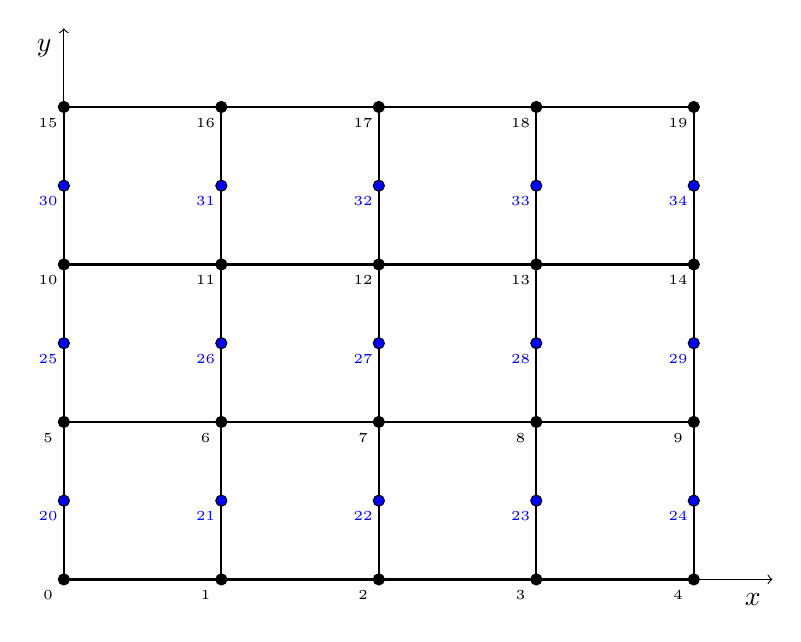
\begin{tikzpicture}
%\draw[fill=gray!23,gray!23](0,0) rectangle (10,8);
%\draw[step=0.5cm,gray,very thin] (0,0) grid (10,8); %background grid

\draw[thick] (1,1) -- (9,1) ;
\draw[thick] (1,3) -- (9,3) ;
\draw[thick] (1,5) -- (9,5) ;
\draw[thick] (1,7) -- (9,7) ;

\draw[thick] (1,1) -- (1,7) ;
\draw[thick] (3,1) -- (3,7) ;
\draw[thick] (5,1) -- (5,7) ;
\draw[thick] (7,1) -- (7,7) ;
\draw[thick] (9,1) -- (9,7) ;

\draw[black,fill=black] (1,1)   circle (2pt);
\draw[black,fill=black] (3,1)   circle (2pt);
\draw[black,fill=black] (5,1)   circle (2pt);
\draw[black,fill=black] (7,1)   circle (2pt);
\draw[black,fill=black] (9,1)   circle (2pt);

\draw[black,fill=black] (1,3)   circle (2pt);
\draw[black,fill=black] (3,3)   circle (2pt);
\draw[black,fill=black] (5,3)   circle (2pt);
\draw[black,fill=black] (7,3)   circle (2pt);
\draw[black,fill=black] (9,3)   circle (2pt);

\draw[black,fill=black] (1,5)   circle (2pt);
\draw[black,fill=black] (3,5)   circle (2pt);
\draw[black,fill=black] (5,5)   circle (2pt);
\draw[black,fill=black] (7,5)   circle (2pt);
\draw[black,fill=black] (9,5)   circle (2pt);

\draw[black,fill=black] (1,7)   circle (2pt);
\draw[black,fill=black] (3,7)   circle (2pt);
\draw[black,fill=black] (5,7)   circle (2pt);
\draw[black,fill=black] (7,7)   circle (2pt);
\draw[black,fill=black] (9,7)   circle (2pt);

\draw[black,fill=blue] (1,2) circle (2pt); 
\draw[black,fill=blue] (3,2) circle (2pt); 
\draw[black,fill=blue] (5,2) circle (2pt); 
\draw[black,fill=blue] (7,2) circle (2pt); 
\draw[black,fill=blue] (9,2) circle (2pt); 

\draw[black,fill=blue] (1,4) circle (2pt); 
\draw[black,fill=blue] (3,4) circle (2pt); 
\draw[black,fill=blue] (5,4) circle (2pt); 
\draw[black,fill=blue] (7,4) circle (2pt); 
\draw[black,fill=blue] (9,4) circle (2pt); 

\draw[black,fill=blue] (1,6) circle (2pt); 
\draw[black,fill=blue] (3,6) circle (2pt); 
\draw[black,fill=blue] (5,6) circle (2pt); 
\draw[black,fill=blue] (7,6) circle (2pt); 
\draw[black,fill=blue] (9,6) circle (2pt); 


\draw[thin,->] (9,1) -- (10,1); %x
\draw[thin,->] (1,7) -- (1,8); %y
\node[] at (9.75,0.75) {$x$};
\node[] at (0.75,7.75) {$y$};

\node[] at (0.8,0.8) {\tiny 0};
\node[] at (2.8,0.8) {\tiny 1};
\node[] at (4.8,0.8) {\tiny 2};
\node[] at (6.8,0.8) {\tiny 3};
\node[] at (8.8,0.8) {\tiny 4};
\node[] at (0.8,2.8) {\tiny 5};
\node[] at (2.8,2.8) {\tiny 6};
\node[] at (4.8,2.8) {\tiny 7};
\node[] at (6.8,2.8) {\tiny 8};
\node[] at (8.8,2.8) {\tiny 9};
\node[] at (0.8,4.8) {\tiny 10};
\node[] at (2.8,4.8) {\tiny 11};
\node[] at (4.8,4.8) {\tiny 12};
\node[] at (6.8,4.8) {\tiny 13};
\node[] at (8.8,4.8) {\tiny 14};
\node[] at (0.8,6.8) {\tiny 15};
\node[] at (2.8,6.8) {\tiny 16};
\node[] at (4.8,6.8) {\tiny 17};
\node[] at (6.8,6.8) {\tiny 18};
\node[] at (8.8,6.8) {\tiny 19};

\node[] at (0.8,1.8) {\tiny \color{blue} 20};
\node[] at (2.8,1.8) {\tiny \color{blue} 21};
\node[] at (4.8,1.8) {\tiny \color{blue} 22};
\node[] at (6.8,1.8) {\tiny \color{blue} 23};
\node[] at (8.8,1.8) {\tiny \color{blue} 24};

\node[] at (0.8,3.8) {\tiny \color{blue} 25};
\node[] at (2.8,3.8) {\tiny \color{blue} 26};
\node[] at (4.8,3.8) {\tiny \color{blue} 27};
\node[] at (6.8,3.8) {\tiny \color{blue} 28};
\node[] at (8.8,3.8) {\tiny \color{blue} 29};

\node[] at (0.8,5.8) {\tiny \color{blue} 30};
\node[] at (2.8,5.8) {\tiny \color{blue} 31};
\node[] at (4.8,5.8) {\tiny \color{blue} 32};
\node[] at (6.8,5.8) {\tiny \color{blue} 33};
\node[] at (8.8,5.8) {\tiny \color{blue} 34};


\end{tikzpicture}\\
\end{center}



iconU:
\begin{verbatim}
           0           1           6           5          20          21
           1           2           7           6          21          22
           2           3           8           7          22          23
           3           4           9           8          23          24
           5           6          11          10          25          26
           6           7          12          11          26          27
           7           8          13          12          27          28
           8           9          14          13          28          29
          10          11          16          15          30          31
          11          12          17          16          31          32
          12          13          18          17          32          33
          13          14          19          18          33          34
\end{verbatim}


\input{python_codes/fieldstone_80/tikz_mesh4x3_v}

iconV:
\begin{verbatim}
           0           1           6           5          20          24
           1           2           7           6          21          25
           2           3           8           7          22          26
           3           4           9           8          23          27
           5           6          11          10          24          28
           6           7          12          11          25          29
           7           8          13          12          26          30
           8           9          14          13          27          31
          10          11          16          15          28          32
          11          12          17          16          29          33
          12          13          18          17          30          34
          13          14          19          18          31          35
\end{verbatim}






\newpage
%%%%%%%%%%%%%%%%%%%%%%%%%%%%%%%%%%
\section{List of subroutines}

 \subsubsection{assign\_values\_to\_qpoints.f90}

 \subsubsection{basis\_functions\_V.f90}
 This file contains 3 functions: 
 \subsubsection{compute\_dNdx\_dNdy\_dNdz.f90}
 This subroutine computes $\partial{\bN^\upnu}/\partial x$, $\partial{\bN^\upnu}/\partial y$ and
 $\partial{\bN^\upnu}/\partial z$ at a location $r,s,t$ passed as argument.
 \subsubsection{compute\_dNdx\_dNdy.f90}
 This subroutine computes $\partial{\bN^\upnu}/\partial x$ and $\partial{\bN^\upnu}/\partial y$
 at a location $r,s$ passed as argument.
 \subsubsection{compute\_dNdx\_dNdy\_dNdz.f90}
 This subroutine computes $\partial{\bN^\uptheta}/\partial x$, 
 $\partial{\bN^\uptheta}/\partial y$ and
 $\partial{\bN^\uptheta}/\partial z$ at a location $r,s,t$ passed as argument.
 \subsubsection{compute\_dNTdx\_dNTdy.f90}
 This subroutine computes $\partial{\bN^\uptheta}/\partial x$ 
 and $\partial{\bN^\uptheta}/\partial y$  at a location $r,s$ passed as argument.
 \subsubsection{compute\_elemental\_matrix\_energy}
 This subroutine buils the elemental matrix ${\bm A}_{el}$ and its corresponding 
 right hand side $\vec{b}_{el}$. 
 \subsubsection{compute\_elemental\_matrix\_stokes.f90}
 Note that when the material model is called directly on the quadrature points and 
 the penalty formulation is used then the viscosity at the reduced quadrature location 
 is obtained by taking the maximum viscosity value carried by the quadrature points of 
 the element. 
 \subsubsection{compute\_elemental\_rho\_eta\_vol}
 This subroutine computes the elemental volume, the average density and 
 viscosity using the values already stored on the quadrature points. 
 \subsubsection{compute\_gravity}

 \subsubsection{compute\_timestep}
 See Section~\ref{ss:cfl}.
 \subsubsection{impose\_boundary\_conditions\_energy}
 This routine takes as argument the elemental matrices and vectors Ael, Bel
 and applies the boundary conditions to them.
 \subsubsection{impose\_boundary\_conditions\_stokes}
 This subroutine modifies the elemental $\K$, $\G$ and $\C$ matrices as well as the 
 elemental rhs $f_{el}$ and $h_{el}$ and returns them modified after imposing
 velocity Dirichlet boundary conditions.
 \subsubsection{template}

 \subsubsection{interpolate\_onto\_nodes.f90}
 This subroutine interpolates the components of the strain rate tensor on the velocity nodes.
 \subsubsection{locate\_point}
 This file contains a few simple subroutines which deal with the localisation of a point 
 in the mesh. The {\tt locate\_point} subroutine receives the coordinates of a point as argument 
 and returns its reduced coordinates and the id of the element it sits in.
 It relies on 3 other subroutines ({\tt find\_ielx\_r}, {\tt find\_iely\_s}, {\tt find\_ielz\_t})
 which take as argument a coorinate (x,y,z) and return the corresponding reduced
 coordinate (r,s,t) and the integer coordinate (ielx,iely,ielz).
 \subsubsection{make\_matrix\_energy}
 This subroutine builds the linear system for the energy equation. 
 It loops over each element, builds its elemental matrix ${\bm A}_{el}$
 and right hand side $\vec{b}_{el}$, applies boundary conditions, 
 and assembles these into the global matrix csrA and the corresponding 
 right hand side rhs\_b. 
 \subsubsection{make\_matrix\_stokes.f90}
 This subroutine loops over all elements, build their elemental matrices and rhs, 
 apply the boundary conditions ont these elemental matrices, and then 
 assembles them in the global matrix, either in CSR or in MUMPS format.
 \subsubsection{matrix\_setup\_A}
 If the geometry is Cartesian then the number of nonzeros in the matrix and its sparsity 
 structures are computed in a very efficient way. 
 \subsubsection{matrix\_setup\_GT.f90}

 \subsubsection{matrix\_setup\_K}

 \subsubsection{matrix\_setup\_M}
 See Section~\ref{ss:symmcsrss}. 
 \subsubsection{output\_mesh.f90}
 This subroutine produces the {\filenamefont meshV.vtu} file which only 
 contains the corner nodes.
 \subsubsection{output\_qpoints}

 \subsubsection{output\_solution}
 This subroutine generates the {\filenamefont solution.vtu} in the {\foldernamefont OUTPUT}
 folder. It also generates the basic ascii file {\filenamefont solution.ascii}
 \subsubsection{output\_swarm.f90}
 This subroutine produces the {\filenamefont swarm.vtu} file in the 
 {\foldernamefont OUTPUT} folder which contains the 
 swarm of particles with all their properties.
 \subsubsection{paint\_swarm}
 
 \subsubsection{pcg\_solver\_csr}
 The subroutine solves $A\cdot = b$ by means f the preconditioned Conjugate Gradient method
 and the implementation follows algorithm 2.2 on page 82 of Elman, Silvester \&
 Wathen \cite{elsw}:
 
 Choose ${\vec u}^{(0)}$, compute ${\vec \phi}^{(0)}={\bm A}\cdot {\vec u}^{(0)}$ 
 then ${\vec r}^{(0)}={\vec f}-{\vec \phi}^{(0)}$, 
 ${\vec z}^{(0)}={\bm M}^{-1}\cdot {\vec r}^{(0)}$ and set ${\vec p}^{(0)}={\vec z}^{(0)}$.
 
 For $k=0$ until convergence do
 \begin{itemize}
 \item ${\vec \phi}^{(k)}={\bm A}\cdot {\vec p}^{(k)}$
 \item compute $\alpha_k = <{\vec z}^{(k)},{\vec r}^{(k)}>/<{\vec \phi}^{(k)},{\vec p}^{(k)}>$
 \item ${\vec u}^{(k+1)}={\vec u}^{(k)}+\alpha_k {\vec p}^{(k)}$
 \item ${\vec r}^{(k+1)}={\vec r}^{(k)}-\alpha_k{\vec \phi}^{(k)}$
 \item test for convergence
 \item ${\vec z}^{(k+1)}=M^{-1} {\vec r}^{(k+1)}$
 \item $\beta_k= <{\vec z}^{(k+1)},{\vec r}^{(k+1)}>/<{\vec z}^{(k)},{\vec r}^{(k)}>$
 \item ${\vec p}^{(k+1)}={\vec z}^{(k+1)}+\beta_k {\vec p}^{(k)}$
 \end{itemize}
 The convergence test is $\| \vec{r}_{k+1} \|_2/ \| \vec{r}_{k+1} \|_2 < tol$, 
 the maximum number of iterations is set to 1000, and the relative tolerance to $tol=10^{-6}$.
 Since the preconditioned is the diagonal of the ${\bm A}$ matrix, then the inverse of 
 ${\bm M}$ is trivial to compute/apply. 
 \subsubsection{postprocessors.f90}
 This subroutine computes the root mean square velocity
 and each of the average velocity components. It also 
 computes the volume using GLQ.
 \subsubsection{prescribe\_stokes\_solution.f90}
 This subroutine prescribes the velocity, pressure, temperature and strain rate components
 on the corners of each element via the {\sl analytical\_solution} subroutine.
 \subsubsection{quadrature\_setup.f90}
 This subroutine allocates all GLQ-related arrays for each element.
 It further computes the real $(x_q,y_q,z_q)$ and reduced $(r_q,s_q,t_q)$
 coordinates of the GLQ points, and assigns them their weights.
 \subsubsection{recover\_pressure\_penalty}
 This is scheme 4 in Section~\ref{psmoothing} (see \stone~12) which was proven to be 
 very cheap and very accurate. 
 The viscosity at the reduced quadrature location 
 is obtained by taking the maximum viscosity value carried by the quadrature points of 
 the element. 
 \subsubsection{set\_default\_values}
 This subroutine assigns default values to many of the global variables.
 \subsubsection{set\_global\_parameters\_pair}

 \subsubsection{setup\_cartesian2D.f90}
 This subroutine assigns to every element the coordinates of the its velocity, pressure,
 and temperature nodes, the velocity, pressure and temperature connectivity arrays,
 the coordinates of its center (xc,yc), its integer coordinates (ielx, iely),
 and its dimensions (hx,hy).
 \begin{center}
 \input{tikz/tikz_3x2_q1}
 \end{center}
 \begin{verbatim}
 elt:  1  | iconV  1  2  6   5  iconP  1
 elt:  2  | iconV  2  3  7   6  iconP  2
 elt:  3  | iconV  3  4  8   7  iconP  3
 elt:  4  | iconV  5  6  10  9  iconP  4
 elt:  5  | iconV  6  7  11  10 iconP  5
 elt:  6  | iconV  7  8  12  11 iconP  6
 \end{verbatim}
 \begin{center}
 \begin{flushright} {\tiny {\color{gray} (tikz\_3x2\_mini.tex)}} \end{flushright}
%~~~~~~~~~~~~~~~~~~~~~~~~~~~~~~~~~~~~~~~~~~~~~~~~~~~~~~~~~~~~~~~~~~~~~~~~~~~~~~~~~~~~~~~~~~~~~~~~~~

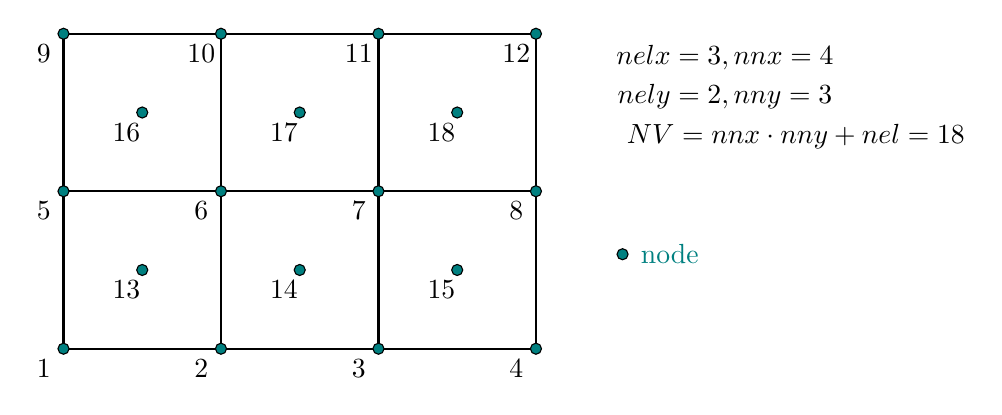
\begin{tikzpicture}
%\draw[step=0.5cm,gray,very thin] (0,0) grid (9,5); %background grid

\draw[thick] (1,1) -- (7,1) -- (7,5) -- (1,5) -- cycle;  
\draw[thick] (1,3) -- (7,3) ;
\draw[thick] (3,1) -- (3,5) ;
\draw[thick] (5,1) -- (5,5) ;

\draw[black,fill=teal] (1,1)     circle (2pt); 
\draw[black,fill=teal] (3,1)     circle (2pt); 
\draw[black,fill=teal] (5,1)     circle (2pt); 
\draw[black,fill=teal] (7,1)     circle (2pt); 

\draw[black,fill=teal] (1,3)     circle (2pt); 
\draw[black,fill=teal] (3,3)     circle (2pt); 
\draw[black,fill=teal] (5,3)     circle (2pt); 
\draw[black,fill=teal] (7,3)     circle (2pt); 

\draw[black,fill=teal] (1,5)     circle (2pt); 
\draw[black,fill=teal] (3,5)     circle (2pt); 
\draw[black,fill=teal] (5,5)     circle (2pt); 
\draw[black,fill=teal] (7,5)     circle (2pt); 

\draw[black,fill=teal] (2,2)     circle (2pt); 
\draw[black,fill=teal] (4,2)     circle (2pt); 
\draw[black,fill=teal] (6,2)     circle (2pt); 
\draw[black,fill=teal] (2,4)     circle (2pt); 
\draw[black,fill=teal] (4,4)     circle (2pt); 
\draw[black,fill=teal] (6,4)     circle (2pt); 

\node[] at (0.75,0.75) {1};
\node[] at (2.75,0.75) {2};
\node[] at (4.75,0.75) {3};
\node[] at (6.75,0.75) {4};

\node[] at (0.75,2.75) {5};
\node[] at (2.75,2.75) {6};
\node[] at (4.75,2.75) {7};
\node[] at (6.75,2.75) {8};

\node[] at (0.75,4.75) {9};
\node[] at (2.75,4.75) {10};
\node[] at (4.75,4.75) {11};
\node[] at (6.75,4.75) {12};

\node[] at (1.8,1.75) {13};
\node[] at (3.8,1.75) {14};
\node[] at (5.8,1.75) {15};
\node[] at (1.8,3.75) {16};
\node[] at (3.8,3.75) {17};
\node[] at (5.8,3.75) {18};

\draw[black,fill=teal] (8.1,2.2) circle (2pt); 
\node[] at (8.7,2.2) {{\color{teal}node}};

\node[] at (9.4,4.7) {$nelx=3, nnx=4$};
\node[] at (9.4,4.2) {$nely=2, nny=3$};
\node[] at (10.3,3.7) {$NV=nnx\cdot nny+nel=18$};

\end{tikzpicture}


 \end{center}
 \begin{verbatim}
 elt:  1  | iconV  1  2  6   5   13 iconP  1  2  6   5
 elt:  2  | iconV  2  3  7   6   14 iconP  2  3  7   6
 elt:  3  | iconV  3  4  8   7   15 iconP  3  4  8   7
 elt:  4  | iconV  5  6  10  9   16 iconP  5  6  10  9
 elt:  5  | iconV  6  7  11  10  17 iconP  6  7  11  10
 elt:  6  | iconV  7  8  12  11  18 iconP  7  8  12  11
 \end{verbatim}
 \begin{center}
 \begin{flushright} {\tiny {\color{gray} (tikz\_3x2\_q2.tex)}} \end{flushright}
%~~~~~~~~~~~~~~~~~~~~~~~~~~~~~~~~~~~~~~~~~~~~~~~~~~~~~~~~~~~~~~~~~~~~~~~~~~~~~~~~~~~~~~~~~~~~~~~~~~

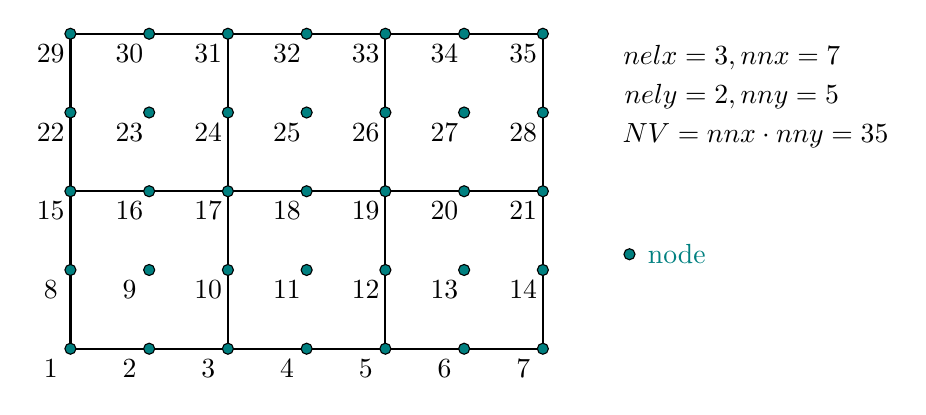
\begin{tikzpicture}
%\draw[step=0.5cm,gray,very thin] (0,0) grid (9,5); %background grid

\draw[thick] (1,1) -- (7,1) -- (7,5) -- (1,5) -- cycle;  
\draw[thick] (1,3) -- (7,3) ;
\draw[thick] (3,1) -- (3,5) ;
\draw[thick] (5,1) -- (5,5) ;

\draw[black,fill=teal] (1,1)     circle (2pt); 
\draw[black,fill=teal] (2,1)     circle (2pt); 
\draw[black,fill=teal] (3,1)     circle (2pt); 
\draw[black,fill=teal] (4,1)     circle (2pt); 
\draw[black,fill=teal] (5,1)     circle (2pt); 
\draw[black,fill=teal] (6,1)     circle (2pt); 
\draw[black,fill=teal] (7,1)     circle (2pt); 

\draw[black,fill=teal] (1,2)     circle (2pt); 
\draw[black,fill=teal] (2,2)     circle (2pt); 
\draw[black,fill=teal] (3,2)     circle (2pt); 
\draw[black,fill=teal] (4,2)     circle (2pt); 
\draw[black,fill=teal] (5,2)     circle (2pt); 
\draw[black,fill=teal] (6,2)     circle (2pt); 
\draw[black,fill=teal] (7,2)     circle (2pt); 

\draw[black,fill=teal] (1,3)     circle (2pt); 
\draw[black,fill=teal] (2,3)     circle (2pt); 
\draw[black,fill=teal] (3,3)     circle (2pt); 
\draw[black,fill=teal] (4,3)     circle (2pt); 
\draw[black,fill=teal] (5,3)     circle (2pt); 
\draw[black,fill=teal] (6,3)     circle (2pt); 
\draw[black,fill=teal] (7,3)     circle (2pt); 

\draw[black,fill=teal] (1,4)     circle (2pt); 
\draw[black,fill=teal] (2,4)     circle (2pt); 
\draw[black,fill=teal] (3,4)     circle (2pt); 
\draw[black,fill=teal] (4,4)     circle (2pt); 
\draw[black,fill=teal] (5,4)     circle (2pt); 
\draw[black,fill=teal] (6,4)     circle (2pt); 
\draw[black,fill=teal] (7,4)     circle (2pt); 

\draw[black,fill=teal] (1,5)     circle (2pt); 
\draw[black,fill=teal] (2,5)     circle (2pt); 
\draw[black,fill=teal] (3,5)     circle (2pt); 
\draw[black,fill=teal] (4,5)     circle (2pt); 
\draw[black,fill=teal] (5,5)     circle (2pt); 
\draw[black,fill=teal] (6,5)     circle (2pt); 
\draw[black,fill=teal] (7,5)     circle (2pt); 

\node[] at (0.75,0.75) {1};
\node[] at (1.75,0.75) {2};
\node[] at (2.75,0.75) {3};
\node[] at (3.75,0.75) {4};
\node[] at (4.75,0.75) {5};
\node[] at (5.75,0.75) {6};
\node[] at (6.75,0.75) {7};

\node[] at (0.75,1.75) {8};
\node[] at (1.75,1.75) {9};
\node[] at (2.75,1.75) {10};
\node[] at (3.75,1.75) {11};
\node[] at (4.75,1.75) {12};
\node[] at (5.75,1.75) {13};
\node[] at (6.75,1.75) {14};

\node[] at (0.75,2.75) {15};
\node[] at (1.75,2.75) {16};
\node[] at (2.75,2.75) {17};
\node[] at (3.75,2.75) {18};
\node[] at (4.75,2.75) {19};
\node[] at (5.75,2.75) {20};
\node[] at (6.75,2.75) {21};

\node[] at (0.75,3.75) {22};
\node[] at (1.75,3.75) {23};
\node[] at (2.75,3.75) {24};
\node[] at (3.75,3.75) {25};
\node[] at (4.75,3.75) {26};
\node[] at (5.75,3.75) {27};
\node[] at (6.75,3.75) {28};

\node[] at (0.75,4.75) {29};
\node[] at (1.75,4.75) {30};
\node[] at (2.75,4.75) {31};
\node[] at (3.75,4.75) {32};
\node[] at (4.75,4.75) {33};
\node[] at (5.75,4.75) {34};
\node[] at (6.75,4.75) {35};

\draw[black,fill=teal] (8.1,2.2) circle (2pt); 
\node[] at (8.7,2.2) {{\color{teal}node}};

\node[] at (9.4,4.7) {$nelx=3, nnx=7$};
\node[] at (9.4,4.2) {$nely=2, nny=5$};
\node[] at (9.7,3.7) {$NV=nnx\cdot nny=35$};

\end{tikzpicture}

 \end{center}
 \begin{verbatim}
 elt:  1  | iconV  1   2   3   8   9   10  15  16  17 iconP           1           2           6           5
 elt:  2  | iconV  3   4   5   10  11  12  17  18  19 iconP           2           3           7           6
 elt:  3  | iconV  5   6   7   12  13  14  19  20  21 iconP           3           4           8           7
 elt:  4  | iconV  15  16  17  22  23  24  29  30  31 iconP           5           6          10           9
 elt:  5  | iconV  17  18  19  24  25  26  31  32  33 iconP           6           7          11          10
 elt:  6  | iconV  19  20  21  26  27  28  33  34  35 iconP           7           8          12          11
 \end{verbatim}
 \subsubsection{setup\_cartesian3D.f90}
 This subroutine assigns to every element the coordinates of the its velocity, pressure,
 and temperature nodes, the velocity, pressure and temperature connectivity arrays,
 the coordinates of its center (xc,yc,zc), its integer coordinates (ielx,iely,ielz),
 and its dimensions (hx,hy,hz).
 \subsubsection{solve\_energy}
 This routine solves the energy equation using a GMRES solver obtained from 
 \url{https://people.sc.fsu.edu/~jburkardt/f_src/mgmres/mgmres.html} 
 \subsubsection{solve\_KV\_eq\_f}
 This subroutine solves the system $\K\cdot \vec{V} = \vec{f}$. The matrix is 
 implicit passed as argument via the module but the rhs and the guess vector are 
 passed as arguments.
 If MUMPS is used the system is solved via MUMPS (the guess is vector
 is then neglected), otherwise a call is made to  the {\tt solve\_cg\_diagprec} subroutine.
 \subsubsection{solve\_stokes}
 This subroutine solves the Stokes system: if it is a saddle point problem 
 it does so using the preconditioned conjugate gradient (PCG) applied 
 to the Schur complement $\SSS$  (see Section~\ref{ss:schurpcg}).
 If the penalty method is used 
 \subsubsection{spmv\_kernels}
 This file contains the Sparse Matrix-Vector multiplication kernels (see Section~\ref{ss:spmv}).
 \subsubsection{swarm\_setup.f90}
 This subroutine generates the swarm of particles. The layout is controled 
 by the {\tt init\_marker\_random} parameter.
 \begin{center}
 \includegraphics[width=5cm]{ELEFANT/images/swarm_reg} 
 \includegraphics[width=5cm]{ELEFANT/images/swarm_rand} 
 \end{center}
 \subsubsection{template}

 \subsubsection{test\_basis\_functions}
 This subroutine tests the consistency of the basis functions. 
 An analytical velocity field is prescribed (constant, linear or quadratic) and the 
 corresponding values are computed onto the quadrature points via the 
 (derivatives of the) basis functions.
 It generates three ascii files in the {\foldernamefont OUTPUT} folder which 
 are to be processed with the gnuplot script present there.
 \subsubsection{write\_stats}














\section{ELEFANT} %%%%%%%%%%%%%%%%%%%%%%%%%%%%%%%%%%%%%%%%%%%%%%%%%%%%%%%%%%%%%%%%%%%%%%%%%%%%%%%%%





























\newpage
%---------------------------------------------------
\subsection{$Q_1\times P_0$ cartesian identity card}

Check Section~\ref{sec:sparse_storage}

\begin{small}
\begin{verbatim}
spaceV='__Q1'
spaceP='__Q0'
nelx=3
nely=2
nel=6
NV=12
NP=6

9------10------11------12     -------------------------
|       |       |       |     |       |       |       |
|       |       |       |     |   4   |   5   |   6   |
|       |       |       |     |       |       |       |
5-------6-------7-------8     |-------|-------|-------|
|       |       |       |     |       |       |       |
|       |       |       |     |   1   |   2   |   3   |
|       |       |       |     |       |       |       | 
1-------2-------3-------4     ------------------------- 

elt: 1  | iconV  1  2   6   5 iconP  1
elt: 2  | iconV  2  3   7   6 iconP  2
elt: 3  | iconV  3  4   8   7 iconP  3
elt: 4  | iconV  5  6  10   9 iconP  4
elt: 5  | iconV  6  7  11  10 iconP  5
elt: 6  | iconV  7  8  12  11 iconP  6

node   1 belongs to  1  elts | 1           0           0           0
node   2 belongs to  2  elts | 1           2           0           0
node   3 belongs to  2  elts | 2           3           0           0
node   4 belongs to  1  elts | 3           0           0           0
node   5 belongs to  2  elts | 1           4           0           0
node   6 belongs to  4  elts | 1           2           4           5
node   7 belongs to  4  elts | 2           3           5           6
node   8 belongs to  2  elts | 3           6           0           0
node   9 belongs to  1  elts | 4           0           0           0
node  10 belongs to  2  elts | 4           5           0           0
node  11 belongs to  2  elts | 5           6           0           0
node  12 belongs to  1  elts | 6           0           0           0

\end{verbatim}
\end{small}

Each elemental K matrix is 8x8

\begin{small}
\[
\begin{array}{cccccccccccccccccccccccccccc}
& u_1 & u_2 & u_3 & u_4 & u_5 & u_6 &
u_7 & u_8 & u_9 & u_{10} & u_{11} & u_{12} 
& v_1 & v_2 & v_3 & v_4 & v_5 & v_6 &
v_7 & v_8 & v_9 & v_{10} & v_{11} & v_{12} \\
u_1 & * & * & && * & * &&&&&&& * & * &&& * & *\\
u_2 & * & * & && * & * &&&&&&& * & * &&& * & *\\
_3
\end{array}
\]
\end{small}










\newpage
%---------------------------------------------------
\subsection{$Q_1\times P_0$ annulus identity card}

\begin{center}
\includegraphics[width=7cm]{images/ELEFANT/annulus_Q1}
\end{center}




\newpage
%---------------------------------------------------
\subsection{$Q_2\times Q_1$ annulus identity card}

\begin{small}
\begin{verbatim}
spaceV='__Q2'
spaceP='__Q1'
nelr=2
nelphi=8
nel=8
NV=80
NP=24
\end{verbatim}
\end{small}

\begin{center}
\includegraphics[width=7cm]{images/ELEFANT/annulus_Q2}
\end{center}

\begin{verbatim}

                 25           15
                 24         14
                 23       13
                 22     12
                 21   11
                  |     
                  |
45 44 43 42 41----+------1-2-3-4-5
\end{verbatim}




\begin{small}
\begin{verbatim}
V node     1 belongs to  2 elts:       1    15     0     0     0     0     0     0
V node     2 belongs to  2 elts:       1    15     0     0     0     0     0     0
V node     3 belongs to  4 elts:       1     2    15    16     0     0     0     0
V node     4 belongs to  2 elts:       2    16     0     0     0     0     0     0
V node     5 belongs to  2 elts:       2    16     0     0     0     0     0     0
V node     6 belongs to  1 elts:       1     0     0     0     0     0     0     0
V node     7 belongs to  1 elts:       1     0     0     0     0     0     0     0
V node     8 belongs to  2 elts:       1     2     0     0     0     0     0     0
V node     9 belongs to  1 elts:       2     0     0     0     0     0     0     0
V node    10 belongs to  1 elts:       2     0     0     0     0     0     0     0
V node    11 belongs to  2 elts:       1     3     0     0     0     0     0     0
V node    12 belongs to  2 elts:       1     3     0     0     0     0     0     0
V node    13 belongs to  4 elts:       1     2     3     4     0     0     0     0
V node    14 belongs to  2 elts:       2     4     0     0     0     0     0     0
V node    15 belongs to  2 elts:       2     4     0     0     0     0     0     0
V node    16 belongs to  1 elts:       3     0     0     0     0     0     0     0
V node    17 belongs to  1 elts:       3     0     0     0     0     0     0     0
V node    18 belongs to  2 elts:       3     4     0     0     0     0     0     0
V node    19 belongs to  1 elts:       4     0     0     0     0     0     0     0
V node    20 belongs to  1 elts:       4     0     0     0     0     0     0     0
V node    21 belongs to  2 elts:       3     5     0     0     0     0     0     0
V node    22 belongs to  2 elts:       3     5     0     0     0     0     0     0
V node    23 belongs to  4 elts:       3     4     5     6     0     0     0     0
V node    24 belongs to  2 elts:       4     6     0     0     0     0     0     0
V node    25 belongs to  2 elts:       4     6     0     0     0     0     0     0
V node    26 belongs to  1 elts:       5     0     0     0     0     0     0     0
V node    27 belongs to  1 elts:       5     0     0     0     0     0     0     0
V node    28 belongs to  2 elts:       5     6     0     0     0     0     0     0
V node    29 belongs to  1 elts:       6     0     0     0     0     0     0     0
V node    30 belongs to  1 elts:       6     0     0     0     0     0     0     0
V node    31 belongs to  2 elts:       5     7     0     0     0     0     0     0
V node    32 belongs to  2 elts:       5     7     0     0     0     0     0     0
V node    33 belongs to  4 elts:       5     6     7     8     0     0     0     0
V node    34 belongs to  2 elts:       6     8     0     0     0     0     0     0
V node    35 belongs to  2 elts:       6     8     0     0     0     0     0     0
V node    36 belongs to  1 elts:       7     0     0     0     0     0     0     0
V node    37 belongs to  1 elts:       7     0     0     0     0     0     0     0
V node    38 belongs to  2 elts:       7     8     0     0     0     0     0     0
V node    39 belongs to  1 elts:       8     0     0     0     0     0     0     0
V node    40 belongs to  1 elts:       8     0     0     0     0     0     0     0
V node    41 belongs to  2 elts:       7     9     0     0     0     0     0     0
V node    42 belongs to  2 elts:       7     9     0     0     0     0     0     0
V node    43 belongs to  4 elts:       7     8     9    10     0     0     0     0
V node    44 belongs to  2 elts:       8    10     0     0     0     0     0     0
V node    45 belongs to  2 elts:       8    10     0     0     0     0     0     0
V node    46 belongs to  1 elts:       9     0     0     0     0     0     0     0
V node    47 belongs to  1 elts:       9     0     0     0     0     0     0     0
V node    48 belongs to  2 elts:       9    10     0     0     0     0     0     0
V node    49 belongs to  1 elts:      10     0     0     0     0     0     0     0
V node    50 belongs to  1 elts:      10     0     0     0     0     0     0     0
V node    51 belongs to  2 elts:       9    11     0     0     0     0     0     0
V node    52 belongs to  2 elts:       9    11     0     0     0     0     0     0
V node    53 belongs to  4 elts:       9    10    11    12     0     0     0     0
V node    54 belongs to  2 elts:      10    12     0     0     0     0     0     0
V node    55 belongs to  2 elts:      10    12     0     0     0     0     0     0
V node    56 belongs to  1 elts:      11     0     0     0     0     0     0     0
V node    57 belongs to  1 elts:      11     0     0     0     0     0     0     0
V node    58 belongs to  2 elts:      11    12     0     0     0     0     0     0
V node    59 belongs to  1 elts:      12     0     0     0     0     0     0     0
V node    60 belongs to  1 elts:      12     0     0     0     0     0     0     0
V node    61 belongs to  2 elts:      11    13     0     0     0     0     0     0
V node    62 belongs to  2 elts:      11    13     0     0     0     0     0     0
V node    63 belongs to  4 elts:      11    12    13    14     0     0     0     0
V node    64 belongs to  2 elts:      12    14     0     0     0     0     0     0
V node    65 belongs to  2 elts:      12    14     0     0     0     0     0     0
V node    66 belongs to  1 elts:      13     0     0     0     0     0     0     0
V node    67 belongs to  1 elts:      13     0     0     0     0     0     0     0
V node    68 belongs to  2 elts:      13    14     0     0     0     0     0     0
V node    69 belongs to  1 elts:      14     0     0     0     0     0     0     0
V node    70 belongs to  1 elts:      14     0     0     0     0     0     0     0
V node    71 belongs to  2 elts:      13    15     0     0     0     0     0     0
V node    72 belongs to  2 elts:      13    15     0     0     0     0     0     0
V node    73 belongs to  4 elts:      13    14    15    16     0     0     0     0
V node    74 belongs to  2 elts:      14    16     0     0     0     0     0     0
V node    75 belongs to  2 elts:      14    16     0     0     0     0     0     0
V node    76 belongs to  1 elts:      15     0     0     0     0     0     0     0
V node    77 belongs to  1 elts:      15     0     0     0     0     0     0     0
V node    78 belongs to  2 elts:      15    16     0     0     0     0     0     0
V node    79 belongs to  1 elts:      16     0     0     0     0     0     0     0
V node    80 belongs to  1 elts:      16     0     0     0     0     0     0     0

P node     1 belongs to  2 elts:       1    15     0     0     0     0     0     0
P node     2 belongs to  4 elts:       1     2    15    16     0     0     0     0
P node     3 belongs to  2 elts:       2    16     0     0     0     0     0     0
P node     4 belongs to  2 elts:       1     3     0     0     0     0     0     0
P node     5 belongs to  4 elts:       1     2     3     4     0     0     0     0
P node     6 belongs to  2 elts:       2     4     0     0     0     0     0     0
P node     7 belongs to  2 elts:       3     5     0     0     0     0     0     0
P node     8 belongs to  4 elts:       3     4     5     6     0     0     0     0
P node     9 belongs to  2 elts:       4     6     0     0     0     0     0     0
P node    10 belongs to  2 elts:       5     7     0     0     0     0     0     0
P node    11 belongs to  4 elts:       5     6     7     8     0     0     0     0
P node    12 belongs to  2 elts:       6     8     0     0     0     0     0     0
P node    13 belongs to  2 elts:       7     9     0     0     0     0     0     0
P node    14 belongs to  4 elts:       7     8     9    10     0     0     0     0
P node    15 belongs to  2 elts:       8    10     0     0     0     0     0     0
P node    16 belongs to  2 elts:       9    11     0     0     0     0     0     0
P node    17 belongs to  4 elts:       9    10    11    12     0     0     0     0
P node    18 belongs to  2 elts:      10    12     0     0     0     0     0     0
P node    19 belongs to  2 elts:      11    13     0     0     0     0     0     0
P node    20 belongs to  4 elts:      11    12    13    14     0     0     0     0
P node    21 belongs to  2 elts:      12    14     0     0     0     0     0     0
P node    22 belongs to  2 elts:      13    15     0     0     0     0     0     0
P node    23 belongs to  4 elts:      13    14    15    16     0     0     0     0
P node    24 belongs to  2 elts:      14    16     0     0     0     0     0     0
\end{verbatim}
\end{small}














\newpage
%---------------------------------------------------
\subsection{$Q_2 \times Q_1$ cartesian identity card}
\begin{small}
\begin{verbatim}
spaceV='__Q2'
spaceP='__Q1'
nelx=3
nely=2
nel=6
NV=7*5=35
NP=12

        V nodes                       elements                     P nodes 

29--30--31--32--33--34--35    -------------------------    9------10------11------12
|       |       |       |     |       |       |       |    |       |       |       |
22  23  24  25  26  27  28    |   4   |   5   |   6   |    |       |       |       |
|       |       |       |     |       |       |       |    |       |       |       |
15--16--17--18--19--20--21    |-------|-------|-------|    5-------6-------7-------8
|       |       |       |     |       |       |       |    |       |       |       |
8   9   10  11  12  13  14    |   1   |   2   |   3   |    |       |       |       |
|       |       |       |     |       |       |       |    |       |       |       |
1---2---3---4---5---6---7     -------------------------    1-------2-------3-------4

elt: 1  | iconV  1 2  3   8  9  10 15 16 17 iconP 1 2 6  5
elt: 2  | iconV  3 4  5   10 11 12 17 18 19 iconP 2 3 7  6
elt: 3  | iconV  5 6  7   12 13 14 19 20 21 iconP 3 4 8  7
elt: 4  | iconV  15 16 17 22 23 24 29 30 31 iconP 5 6 10 9
elt: 5  | iconV  17 18 19 24 25 26 31 32 33 iconP 6 7 11 10
elt: 6  | iconV  19 20 21 26 27 28 33 34 35 iconP 7 8 12 11

a node belongs to at most 4 elements:

V node     1 belongs to  1 elts:       1     0     0     0     0     0     0     0
V node     2 belongs to  1 elts:       1     0     0     0     0     0     0     0
V node     3 belongs to  2 elts:       1     2     0     0     0     0     0     0
V node     4 belongs to  1 elts:       2     0     0     0     0     0     0     0
V node     5 belongs to  2 elts:       2     3     0     0     0     0     0     0
V node     6 belongs to  1 elts:       3     0     0     0     0     0     0     0
V node     7 belongs to  1 elts:       3     0     0     0     0     0     0     0
V node     8 belongs to  1 elts:       1     0     0     0     0     0     0     0
V node     9 belongs to  1 elts:       1     0     0     0     0     0     0     0
V node    10 belongs to  2 elts:       1     2     0     0     0     0     0     0
V node    11 belongs to  1 elts:       2     0     0     0     0     0     0     0
V node    12 belongs to  2 elts:       2     3     0     0     0     0     0     0
V node    13 belongs to  1 elts:       3     0     0     0     0     0     0     0
V node    14 belongs to  1 elts:       3     0     0     0     0     0     0     0
V node    15 belongs to  2 elts:       1     4     0     0     0     0     0     0
V node    16 belongs to  2 elts:       1     4     0     0     0     0     0     0
V node    17 belongs to  4 elts:       1     2     4     5     0     0     0     0
V node    18 belongs to  2 elts:       2     5     0     0     0     0     0     0
V node    19 belongs to  4 elts:       2     3     5     6     0     0     0     0
V node    20 belongs to  2 elts:       3     6     0     0     0     0     0     0
V node    21 belongs to  2 elts:       3     6     0     0     0     0     0     0
V node    22 belongs to  1 elts:       4     0     0     0     0     0     0     0
V node    23 belongs to  1 elts:       4     0     0     0     0     0     0     0
V node    24 belongs to  2 elts:       4     5     0     0     0     0     0     0
V node    25 belongs to  1 elts:       5     0     0     0     0     0     0     0
V node    26 belongs to  2 elts:       5     6     0     0     0     0     0     0
V node    27 belongs to  1 elts:       6     0     0     0     0     0     0     0
V node    28 belongs to  1 elts:       6     0     0     0     0     0     0     0
V node    29 belongs to  1 elts:       4     0     0     0     0     0     0     0
V node    30 belongs to  1 elts:       4     0     0     0     0     0     0     0
V node    31 belongs to  2 elts:       4     5     0     0     0     0     0     0
V node    32 belongs to  1 elts:       5     0     0     0     0     0     0     0
V node    33 belongs to  2 elts:       5     6     0     0     0     0     0     0
V node    34 belongs to  1 elts:       6     0     0     0     0     0     0     0
V node    35 belongs to  1 elts:       6     0     0     0     0     0     0     0

P node     1 belongs to  1 elts:       1     0     0     0     0     0     0     0
P node     2 belongs to  2 elts:       1     2     0     0     0     0     0     0
P node     3 belongs to  2 elts:       2     3     0     0     0     0     0     0
P node     4 belongs to  1 elts:       3     0     0     0     0     0     0     0
P node     5 belongs to  2 elts:       1     4     0     0     0     0     0     0
P node     6 belongs to  4 elts:       1     2     4     5     0     0     0     0
P node     7 belongs to  4 elts:       2     3     5     6     0     0     0     0
P node     8 belongs to  2 elts:       3     6     0     0     0     0     0     0
P node     9 belongs to  1 elts:       4     0     0     0     0     0     0     0
P node    10 belongs to  2 elts:       4     5     0     0     0     0     0     0
P node    11 belongs to  2 elts:       5     6     0     0     0     0     0     0
P node    12 belongs to  1 elts:       6     0     0     0     0     0     0     0

csrK%NZ=885

node 1 'sees' nodes 1,2,3,8,9,10,15,16,17, so there will be 18 entries on 1st,2nd lines,
node 2 'sees' nodes 1,2,3,8,9,10,15,16,17, so there will be 18 entries on 3rd,4th line,
node 3 'sees' nodes 1,2,3,4,5,8,9,10,11,12,15,16,17,18,19 so there will be 30 entries on 3rd line, etc ...

            
csrK%ia=           1          19          36          52          67          93
                 118         134         149         175         200         216
                 231         245         258         270         281         291
                 300         316         331         341         350         366
                 381         391         400         408         415         433
                 450         466         481         507         532         548
                 563         589         614         630         645         659
                 672         684         695         705         714         730
                 745         755         764         780         795         805
                 814         822         829         835         840         844
                 847         853         858         862         865         871
                 876         880         883         885         886

P node 1   sees V nodes 1 2 3 8 9 10 15 16 17 | 9
P node 2   sees V nodes 1 2 3 4 5 8 9 10 11 12 15 16 17 18 19 | 15
P node 3   sees V nodes 3 4 5 6 7 10 11 12 13 14 17 18 19 20 21 | 15
P node 4   sees V nodes 5 6 7 12 13 14 19 20 21 | 9
P node 5   sees V nodes 1 2 3 8 9 10 15 16 17 22 23 24 29 30 31 | 15
P node 6   sees V nodes 1 2 3 4 5 8 9 10 11 12 15 16 17 18 19 22 23 24 25 26 29 30 31 32 33 | 25
P node 7   sees V nodes 3 4 5 6 7 10 11 12 13 14 17 18 19 20 21 24 25 26 27 28 31 32 33 34 35 | 25
P node 8   sees V nodes 5 6 7 12 13 14 19 20 21 26 27 28 33 34 35 | 15 
P node 9   sees V nodes 15 16 17 22 23 24 29 30 31 | 9
P node 10  sees V nodes 15 16 17 18 19 22 23 24 25 26 29 30 31 32 33 | 15 
P node 11  sees V nodes 17 18 19 20 21 24 25 26 27 28 31 32 33 34 35 | 15
P node 12  sees V nodes 19 20 21 26 27 28 33 34 35 | 9

csrGT%NZ=(4*9+6*15+2*25=36+90+50)*2=176*2=352

\end{verbatim}
\end{small}

















\newpage
%%%%%%%%%%%%%%%%%%%%%%%%%%%%%%%%%%
\section{The tests}



default parameters




\begin{tabular}{lcccccc}
test & nelx & nely & spaceV & spaceP & inner\_solver\_type & outer\_solver \\
001  &    3 &    2 &     Q1 &     Q0 &                y12m &               \\ 
\end{tabular}


















\newpage
%%%%%%%%%%%%%%%%%%%%%%%%%%%%%%%%%%
\section{The modules and objects}
The whole code is built around a few modules and objects:

\begin{itemize}
\item {\filenamefont module\_parameters.f90}\\
\lstinputlisting[language=Fortran,basicstyle=\tiny]{ELEFANT/module_parameters.f90}

\item {\filenamefont module\_gravity.f90}\\
\lstinputlisting[language=Fortran]{ELEFANT/module_gravity.f90}

\item {\filenamefont module\_materials.f90}\\
\lstinputlisting[language=Fortran]{ELEFANT/module_materials.f90}

\item {\filenamefont module\_mesh.f90}\\
\lstinputlisting[language=Fortran,basicstyle=\tiny]{ELEFANT/module_mesh.f90}

\item {\filenamefont module\_sparse.f90}\\
\lstinputlisting[language=Fortran]{ELEFANT/module_sparse.f90}

\item {\filenamefont module\_statistics.f90}\\
\lstinputlisting[language=Fortran]{ELEFANT/module_statistics.f90}

\item {\filenamefont module\_swarm.f90}\\
\lstinputlisting[language=Fortran]{ELEFANT/module_swarm.f90}

\item {\filenamefont module\_timing.f90}\\
\lstinputlisting[language=Fortran]{ELEFANT/module_timing.f90}

\item {\filenamefont module\_constants.f90}\\
\lstinputlisting[language=Fortran]{ELEFANT/module_constants.f90}

\item {\filenamefont module\_arrays.f90}\\
\lstinputlisting[language=Fortran]{ELEFANT/module_arrays.f90}
\end{itemize}

%%%%%%%%%%%%%%%%%%%%%%%%%%%%%%%%%%
\section{Install MUMPS (Ubuntu)}

\subsection{Sequential install}

Go to the MUMPS website \url{http://mumps.enseeiht.fr/index.php?page=home} and 
fill the form of the Download page. 
Once you have received a link to {\filenamefont MUMPS\_3.X.X.tar.gz}, download
the file and place it in a folder on your computer. Expand it. 
In the terminal place go to the folder, then type:
\begin{verbatim}
> cp Make.inc/Makefile.inc.generic.SEQ Makefile.inc
\end{verbatim}
Edit {\filenamefont Makefile.inc} and replace the C compiler {\tt cc} 
and Fortran compiler {\tt f90} by the names of the compilers on 
your system (in my case {\tt gcc} and {\tt gfortran} respectively).

Then simply make:
\begin{verbatim}
> make 
\end{verbatim}
In the end you should find the following files in the {\tt lib} folder:
\begin{verbatim}
> cd lib
> ls -la
libdmumps.a
libmumps_common.a
libpord.a
\end{verbatim}
Finally copy {\tt libseq/mpif.h} in the \elefant folder.

Edit the Makefile of \elefant to adjust the location of the MUMPS solver.

ADD METIS support


copy dmumps\_struc.h and dmumps\_root.h to main elefant folder.


\subsection{Parallel install}



%%%%%%%%%%%%%%%%%%%%%%%%%%%%%%%%%%
\section{Setting up an experiment/benchmark/cookbook}

opla

\begin{center}
\begin{flushright} {\tiny {\color{gray} (tikz\_elefant\_boundaries.tex)}} \end{flushright}
%~~~~~~~~~~~~~~~~~~~~~~~~~~~~~~~~~~~~~~~~~~~~~~~~~~~~~~~~~~~~~~~~~~~~~~~~~~~~~~~~~~~~~~~~~~~~~~~~~~

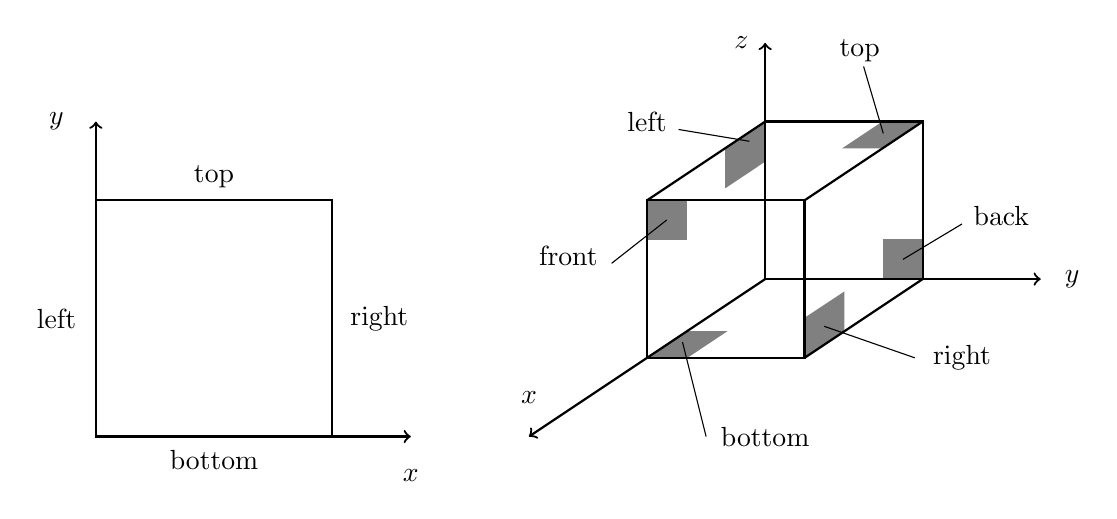
\begin{tikzpicture}
%\draw[step=0.5cm,gray,very thin] (0,0) grid (14,10); %background grid

%2D%%%%%%%%%%%%%%%%%%%%%%%%%%%%%%%%%%%%%%%%%%%%%%%%%%%%%%%%%%%%%%55

\draw[thick] (1,1) -- (4,1) -- (4,4) -- (1,4) -- cycle;  
\draw[thick,->] (1,1)--(5,1);
\draw[thick,->] (1,1)--(1,5);
\node[] at (5,0.5) {$x$};
\node[] at (0.5,5) {$y$};

\node[] at (0.5,2.5) {left};
\node[] at (4.6,2.5) {right};
\node[] at (2.5,0.7) {bottom};
\node[] at (2.5,4.3) {top};

%3d%%%%%%%%%%%%%%%%%%%%%%%%%%%%%%%%%%%%%%%%%%%%%%%%%%%%%%%%%%%%%5

\draw[fill=gray,gray] (8,3.5)--(8.5,3.5)--(8.5,4)--(8,4)--cycle; %front
\draw[fill=gray,gray] (11,3)--(11.5,3)--(11.5,3.5)--(11,3.5)--cycle; %back
\draw[fill=gray,gray] (8,2)--(8.5,2)--(9,2.3333)--(8.5,2.3333)--cycle; %bottom
\draw[fill=gray,gray] (10.5,4.6666)--(11,4.6666)--(11.5,5)--(11,5)--cycle; %top
\draw[fill=gray,gray] (10,2)--(10.5,2.333)--(10.5,2.83)--(10,2.5)--cycle; %right
\draw[fill=gray,gray] (9,4.166)--(9.5,4.5)--(9.5,5)--(9,4.666)--cycle; %left

\draw[thick] (8,2) -- (10,2) -- (10,4) -- (8,4) -- cycle;  
\draw[thick] (9.5,3) -- (11.5,3) -- (11.5,5) -- (9.5,5) -- cycle;  
\draw[thick] (8,4) -- (9.5,5);
\draw[thick] (10,4) -- (11.5,5);
\draw[thick] (10,2) -- (11.5,3);

\draw[thick,->] (9.5,3)--(6.5,1);
\draw[thick,->] (9.5,3)--(9.5,6);
\draw[thick,->] (9.5,3)--(13,3);

\node[] at (8,5) {left};
\node[] at (12,2) {right};
\node[] at (9.5,1) {bottom};
\node[] at (10.7,5.9) {top};
\node[] at (7,3.3) {front};
\node[] at (12.5,3.8) {back};

\node[] at (6.5,1.5) {$x$};
\node[] at (13.4,3) {$y$};
\node[] at (9.2,6) {$z$};

\draw[] (8.75,1)--(8.45,2.2); %bottom
\draw[] (10.25,2.4)--(11.4,2); %right
\draw[] (11.25,3.25)--(12,3.7); %back
\draw[] (10.75,5.7)--(11,4.85); %top
\draw[] (7.55,3.2)--(8.25,3.75); %front
\draw[] (8.4,4.9)--(9.3,4.75); %left

\end{tikzpicture}


\end{center}

%%%%%%%%%%%%%%%%%%%%%%%%%%%%%%%%%%
\section{To do list}

\begin{itemize}
\item explore whether ilu preconditioner is necessary for energy equation.
\item (Reverse) Cuthill-MacKee algorithm, Sloan algorithm ?
\item finish/validate pressure and velocity(ndof=1?) mass matrix 
\end{itemize}




%%%%%%%%%%%%%%%%%%%%%%%%%%%%%
\section{How to install LAPACK}

\begin{verbatim}
mkdir lapack-Sandbox 
cd lapack-sandbox
git clone https://github.com/Reference-LAPACK/lapack.git
mkdir lapack-build
cd lapack-build
cmake ../lapack
make
\end{verbatim}
You will find in /lib the desired libblas.a and liblapack.a libraries.


%%%%%%%%%%%%%%%%%%%%%%%%%%%%%
\section{The MUMPS solver}

MUMPS stands for MUltifrontal Massively Parallel Solver. It is a software package 
for solving systems of linear equations of the 
form ${\bm A}\cdot{\vec x} = {\vec b}$, where ${\bm A}$ is a square sparse matrix (unsymmetric, 
symmetric positive definite, or general symmetric). 

MUMPS implements a direct method which performs a direct factorisation
${\bm A} = {\bm L}\cdot{\bm U}$ where ${\bm L}$ is a lower triangular matrix and ${\bm U}$ 
an upper triangular matrix. If the matrix is symmetric then the factorisation becomes
${\bm A} = {\bm L}\cdot{\bm D}\cdot{\bm L}^T$
where ${\bm D}$ is a block diagonal matrix. 
All the features of the MUMPS package are documented in the manual available from the 
website\footnote{\url{http://mumps.enseeiht.fr/index.php?page=home}}.

%The main features of the MUMPS package include the solution of the transposed system, 
%input of the matrix in assembled format (distributed or centralized) or elemental format, 
%error analysis, iterative refinement, scaling of the original matrix, out-of-core capability, 
%parallel analysis, detection of null pivots, basic estimate of rank deficiency and null space 
%basis for symmetric matrices and computation of a Schur complement matrix. 

MUMPS offers several built-in ordering algorithms as well as an 
interface to external ordering packages such as PORD \cite{schu01}, SCOTCH \cite{pell07} 
or METIS \cite{kaku98} (used in this study). 
The software is mainly written in Fortran 90 although a C interface is available. 
The parallel version of MUMPS requires 
MPI \cite{snoh96} for message passing and makes use of the BLAS \cite{dodd90a,dodd90b}, BLACS, and ScaLAPACK
\cite{blcc97} libraries. 
The sequential version only relies on BLAS and LAPACK.

The system ${\bm A}\cdot{\vec x} = {\vec b}$ is solved in three main steps:
\begin{itemize}
\item Analysis: preprocessing including an 
ordering based on the symmetrized pattern ${\bm A} + {\bm A}^T$ 
and a symbolic factorisation is performed. 

\item Factorisation: a direct factorisation ${\bm A}_{pre} = {\bm L}\cdot{\bm U}$ 
or ${\bm A}_{pre} = {\bm L}\cdot{\bm D}\cdot {\bm L}^T$ depending on 
the symmetry of the preprocessed matrix is computed. 

\item Solution:
The solution of ${\bm L}\cdot{\bm U}\cdot{\vec x}_{pre} = {\vec b}_{pre}$ 
or ${\bm L}\cdot{\bm D}\cdot{\bm L}^T {\vec x}_{pre} = {\vec b}_{pre}$ (where 
${\vec x}_{pre}$ and ${\vec b}_{pre}$ are respectively the transformed solution 
${\vec x}$ and right-hand side ${\vec b}$ associated to the preprocessed matrix 
${\bm A}_{pre}$), is obtained through a forward elimination step
${\bm L}\cdot{\vec y}={\vec b}_{pre}$ (or ${\bm L}\cdot{\bm D}\cdot{\vec y}={\vec b}_{pre}$), 
followed by a backward elimination step
${\bm U}\cdot{\vec x}_{pre} ={\vec y}$ (or ${\bm L}^T{\vec x}_{pre} ={\vec y}$). 

\end{itemize}



%%%%%%%%%%%%%%%%%%%%%%%%%%%%%%%%%%
\section{How we use MUMPS - the elemental format}

What follows is written with $Q_1\times P_0$ elements in mind. 

In two dimensions, the FE grid is composed of $nelx \times nely=nel$ elements. 
The resulting matrix size $N$ is given by $N=(nelx+1)(nely+1)ndofV$ with $ndofV=2$ in 2D.
The connectivity array $icon$ is defined and computed at the beginning for each element. 

The entries $mesh(iel)\%icon(1:4)$ list the nodes making up the element $iel$.
In three dimensions, the grid is naturally composed of 
$nelx \times nely \times nelz = nel$ elements and the 
resulting matrix size is $N=(nelx+1)(nely+1)(nelz+1)ndofV$ with $ndofV=3$.

%------------------------------
\subsection{Allocating arrays}

First, a variable of type {\tt dmumps\_struc} must be declared:
\begin{verbatim}
type(DMUMPS_STRUC) idV 
\end{verbatim}

At the beginning of the program, it is necessary to 
initialise an MPI communicator:

\begin{verbatim}
call mpi_init(ierr)                            
call mpi_comm_size(mpi_comm_world,nproc,ierr) 
call mpi_comm_rank(mpi_comm_world,iproc,ierr) 
\end{verbatim}

Several components of the {\tt idV} variable must then be set and MUMPS 
must be initialised: 
\begin{verbatim}
idV%COMM = MPI_COMM_WORLD 
idV%SYM = 1              
idV%PAR=1                
idV%JOB = -1             
call DMUMPS(idV)        
\end{verbatim}

In the code above
{\tt SYM=1} indicates that the global assembled matrix is symmetric.
{\tt JOB=-1} initializes an instance of the package. 
%Note that a call with 
%{\tt JOB=-1} must be performed before any other call to the package on the same instance. 
%It sets default values for other components of {\tt MUMPS\_STRUC}.
{\tt PAR} must be initialized on all processors and are accessed by MUMPS only during the initialisation phase.
It is here set to 1, i.e. the host is involved in factorisation/solve phases.

In order to solve the FEM problem with MUMPS the user has to declare/build 
a subset of the variables and arrays of {\tt idV} (Note: what follows is only valid in 
the case of an elemental input of the FEM matrix):
\begin{itemize}
\item {\tt idV\%N} is the order of the matrix ${\bm A}$
and {\tt idV\%NELT} is the number of elements being input:
\begin{verbatim}
idV%N=Nfem    
idV%NELT=nel
\end{verbatim}

\item {\tt idV\%ELTPTR} is an integer array of 
length {\tt idV\%NELT+1}. {\tt idV\%ELTPTR(j)} points to the position in {\tt idV\%ELTVAR}
of the first variable in element {\tt j}, and {\tt idV\%ELTPTR(NELT+1)} must be set to 
the position after the last variable of the last element. It is built as follows: 

\begin{lstlisting}
allocate(idV%ELTPTR(idV%NELT+1))
do iel=1,nel                         
   idV%ELTPTR(iel)=1+(iel-1)*(ndofV*mV)   
end do                         
idV%ELTPTR(iel)=1+nel*(ndofV*mV) 
\end{lstlisting}
where $mV=4$ is the number of nodes of the two-dimensional bi-linear $Q_1$ element.

\begin{center}
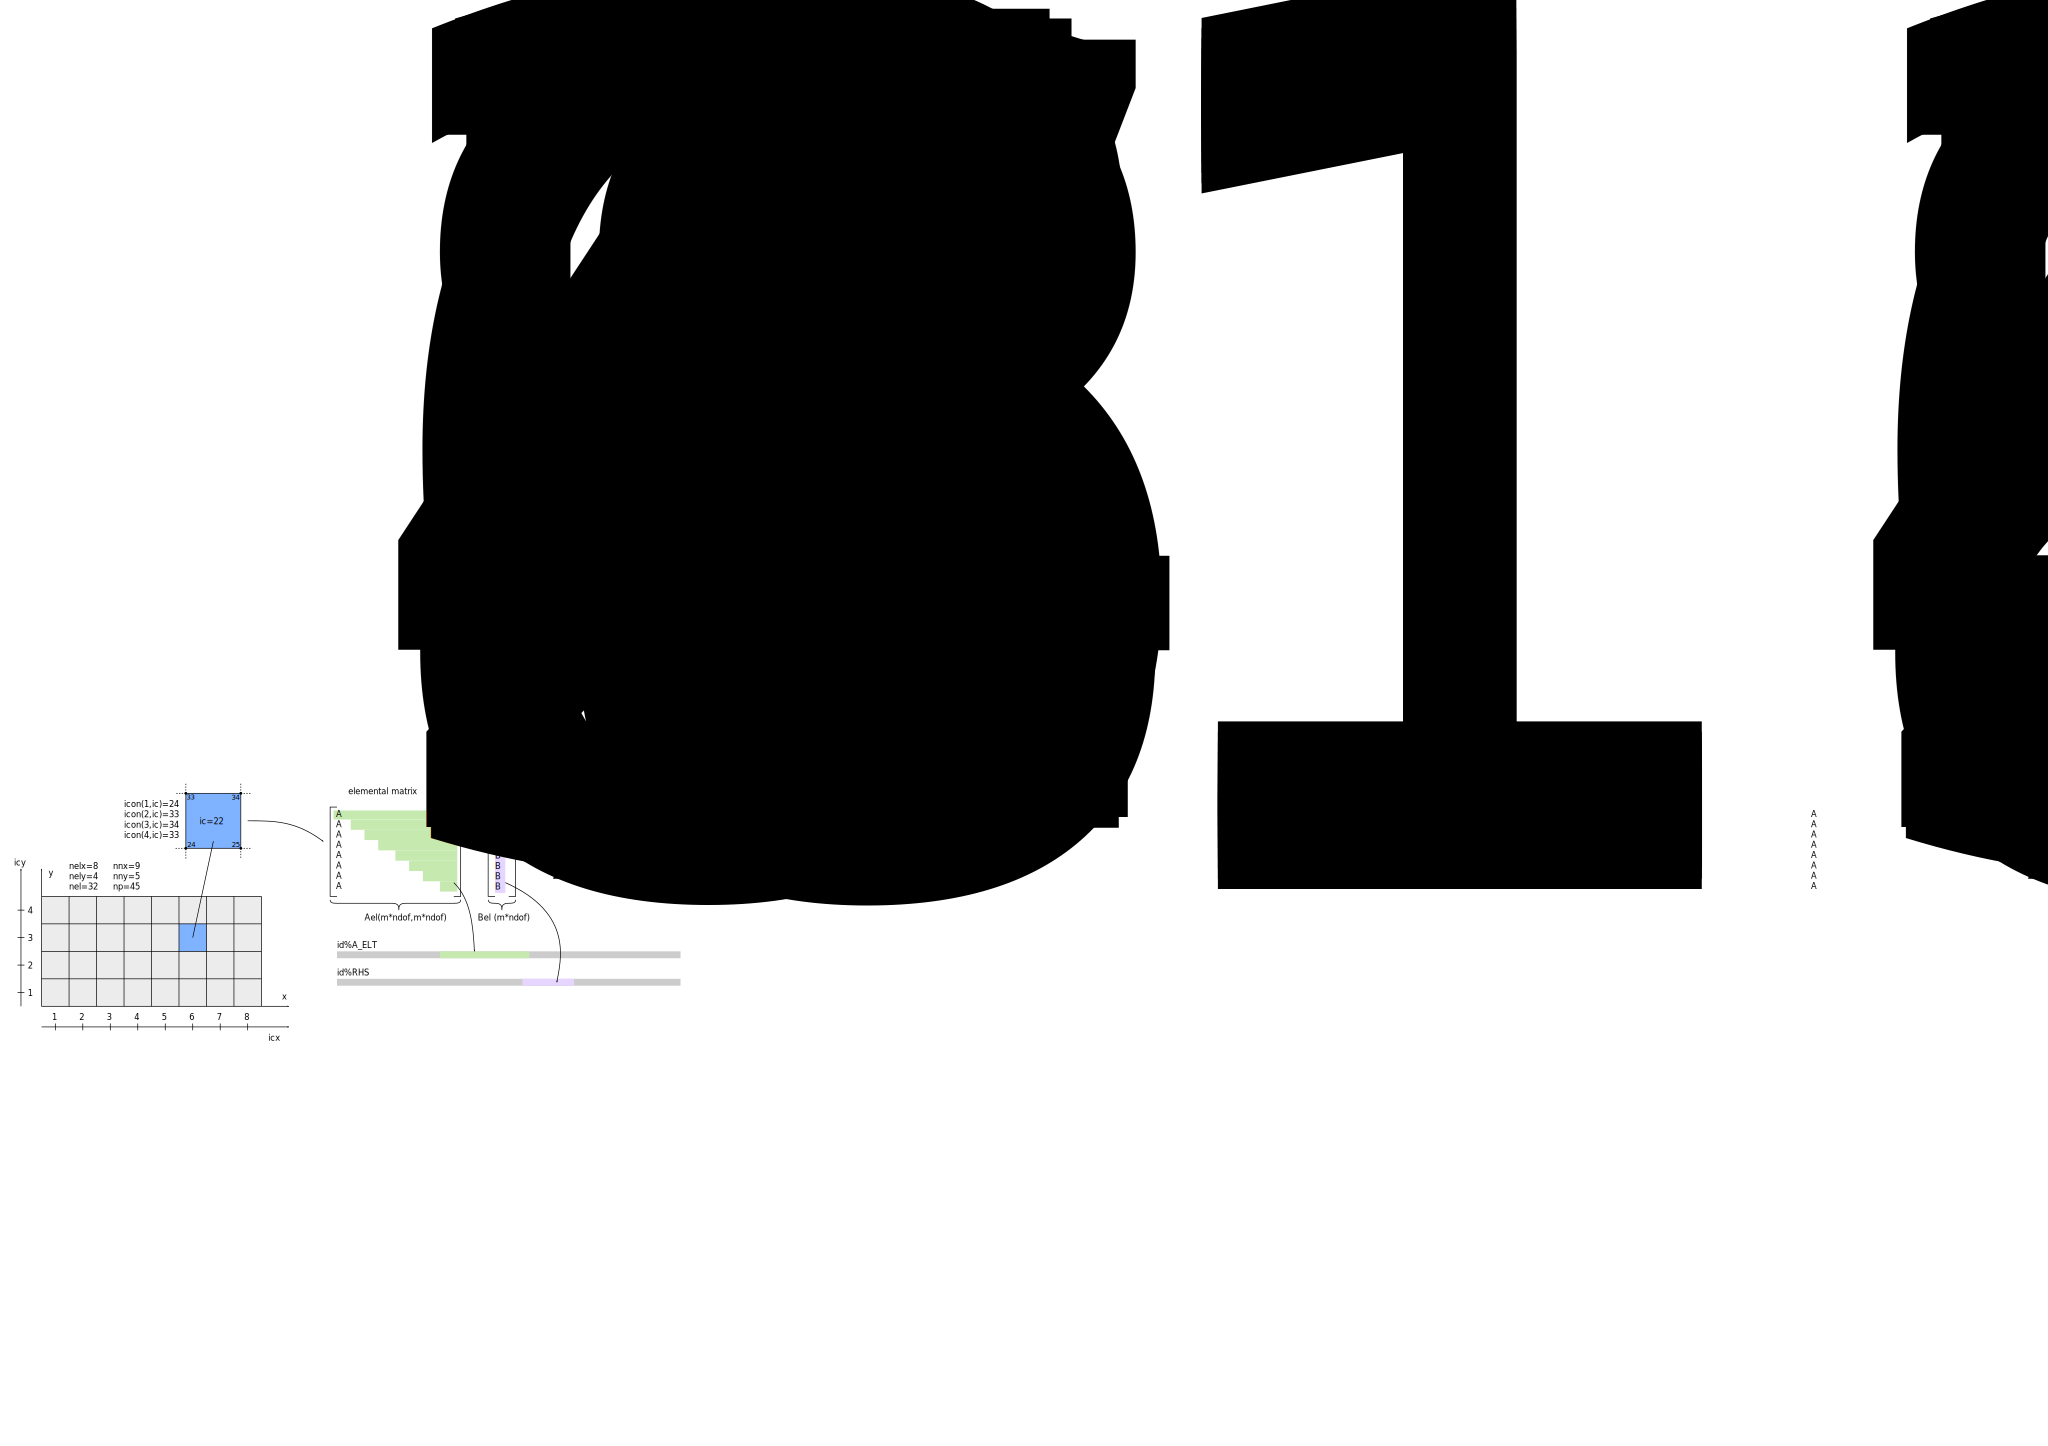
\includegraphics[width=16cm]{images/MUMPS/grid}\\
{\captionfont Schematic representation of an $8\times4$ FE grid. 
Element 22 is singled out, and is shown to
be composed of 4 nodes: 24, 25, 33 and 34. To the right are shown the corresponding elemental
matrix {\tt K\_el} and right hand side {b\_el}, and where the values will be written in the
{\tt idV\%A\_ELT} and {\tt idV\%RHS} arrays respectively.}
\end{center}


\item {\tt idV\%ELTVAR} is an integer array of length {\tt idV\%ELTPTR(NELT+1)-1} and must 
be set to the lists of variables of the elements. 
Those for element {\tt j} are stored in positions {\tt idV\%ELTPTR(j),..., idV\%ELTPTR(j+1)-1}. 
\begin{verbatim}
LELTVAR=nel*(mV*ndofV)  
allocate(idV%ELTVAR(LELTVAR))
counter=0   
do iel=1,nel 
   do k=1,mV    
      inode=mesh(iel)%icon(k)  
      do idof=1,ndof    
         iii=(inode-1)*ndofV+idof   
         counter=counter+1         
         idV%ELTVAR(counter)=iii   
      end do                   
   end do                 
end do               
\end{verbatim}


\item {\tt idV\%A\_ELT} contains the entries of the elemental matrices stored after one another. Since  
all elemental matrices are symmetric one only needs to store the upper half (including the diagonal terms), 
as shown in green colour in the figure above.
Each elemental matrix contains ({\tt mV*ndofV})$\times$({\tt mV*ndofV}) values but only 
({\tt mV*ndofV})({\tt mV*ndofV+1}){\tt /2} will be stored:
\begin{verbatim}
NA_ELT=nel*(mV*ndofV)*(mV*ndofV+1)/2 
allocate(idV%A_ELT (NA_ELT))
\end{verbatim}

\item {\tt RHS} is a real array containing the assembled right-hand side of the linear system:
\begin{verbatim}
allocate(idV%RHS (idV%N))
\end{verbatim}

\end{itemize}

Note that the above code requires little to no change in the case that higher-order elements are used. 

%==================
\subsection{Assembly}

The host loops over the elements and for each element
the matrix ${\bm K}_{el}$. 
 For each element an elemental matrix {\tt K\_el} and a rhs term {\tt b\_el}
are built. Boundary conditions are then applied, 
and half of {\tt K\_el} is then stored in {\tt A\_ELT} while 
{\tt b\_el} is assembled in the global vector {\tt RHS}.

\begin{verbatim}
counter=0
do iel=1,nel

[build elemental matrices K\_el and Bel]
[impose boundary conditions on K\_el, Bel]

do k1=1,m
   ik=icon(k1,iel)
   do i1=1,ndof
      ikk=ndof*(k1-1)+i1
      m1=ndof*(ik-1)+i1
      do k2=1,m
         do i2=1,ndof
            jkk=ndof*(k2-1)+i2
            if (jkk>=ikk) then
            counter=counter+1
            idV%A_ELT(counter)=K_el(ikk,jkk)
            end if
         end do
      end do
      idV%RHS(m1)=idV%RHS(m1)+Bel(ikk)
   end do
end do

end do
\end{verbatim}




%------------------------------
\subsection{Solving the system}

Once the loop over all elements is completed, {\tt INCTL(5)}
must be set to 1 since the elemental format is being used. 
All three phases of the solve are then carried out. Note that the 
vector {\tt RHS} is overriden by the solution after the solve is completed.   

\begin{verbatim}
id%ICNTL(5) = 1 ! choosing elemental format
id%ICNTL(7) = 5 ! using Metis
id%JOB = 1      ! analysis phase 
CALL DMUMPS(id)
id%JOB = 2      ! factorisation phase 
CALL DMUMPS(id)
id%JOB = 3      ! solve phase
CALL DMUMPS(id)
\end{verbatim}

Finally all arrays of the {\tt idV} structure are deallocated:
\begin{verbatim}
deallocate(idV%A_ELT)
deallocate(idV%RHS)
deallocate(idV%ELTPTR)
deallocate(idV%ELTVAR)
\end{verbatim}


 \label{chapt:elefant} %%%%%%%%%%%%%%%%%%%%%%%%%%%%%%%%%%%%%%%%%%%%%%%%%%%

\printbibliography
\end{document}
%%%%%%%%%%%%%%%%%%%%%%%%%%%%%%%%%%%%%%%%%%%%%%%%%%%%%%%%%%%
